\section{OD Construction and Installation} \label{sec:od_construction_sec}

\par
The author spend a total of 15-months in the United States as part of this thesis, the majority of which was spent on-site at SURF for both the TPC and OD construction and installation.
It should be noted that due to COVID-19, the schedule for the installation was severely delayed (18+ months).
In this section, the contributions to the OD installation are described (primarily through photographs), along with design changes that occurred during installation.

\par
The acrylic tanks used to hold the GdLS, created by Reynolds (CITE XXX), were originally designed to be 2.54cm thick, however, the curved moulds used could not provide the accuracy to maintain this requirement, and therefore the thickness of acrylic varied by as much as XXX cm, affecting the structural integrity of the tanks.
The acrylic tanks were bonded together and sealed before being transported to SURF.

\par
Once at SURF, the SATs were transported underground and into the water tank before the OCV, in 2019, as planned in the TDR \cite{LZ_TechnicalDesignReview_ref}.
Then they remained in the water tank as shown in Figure XXX for X months until the OD installation was ready to begin in XXX 2020. 


\par
The TATs were first brought underground in August 2019 for a fit test on top of the OCV (before the ICV has been installed inside).
During the cage journey underground, the tanks valves were opened so that the pressure change would not damage them.
As such, once at the 4850 level, each tank was subjected to a N2 purge to remove as much of the cavern air as possible for the reasons described in Section XXX.
An example of this process is shown in Figure \ref{fig:TAT_purging}.
During this process, it was discovered that the top acrylic sheet had come away from the bond holding it to the side acrylic pieces.
This was later re-bonded, but is mentioned as it meant that the tank was exposed to cavern air for a prolonged period of time.
Additionally, during the fit test, it was found that the curvature of the TATs differed from the OCV which would leave a large water-gap between the two, increasing the probability of hydrogen neutron capture.

\begin{figure}[!htbp]
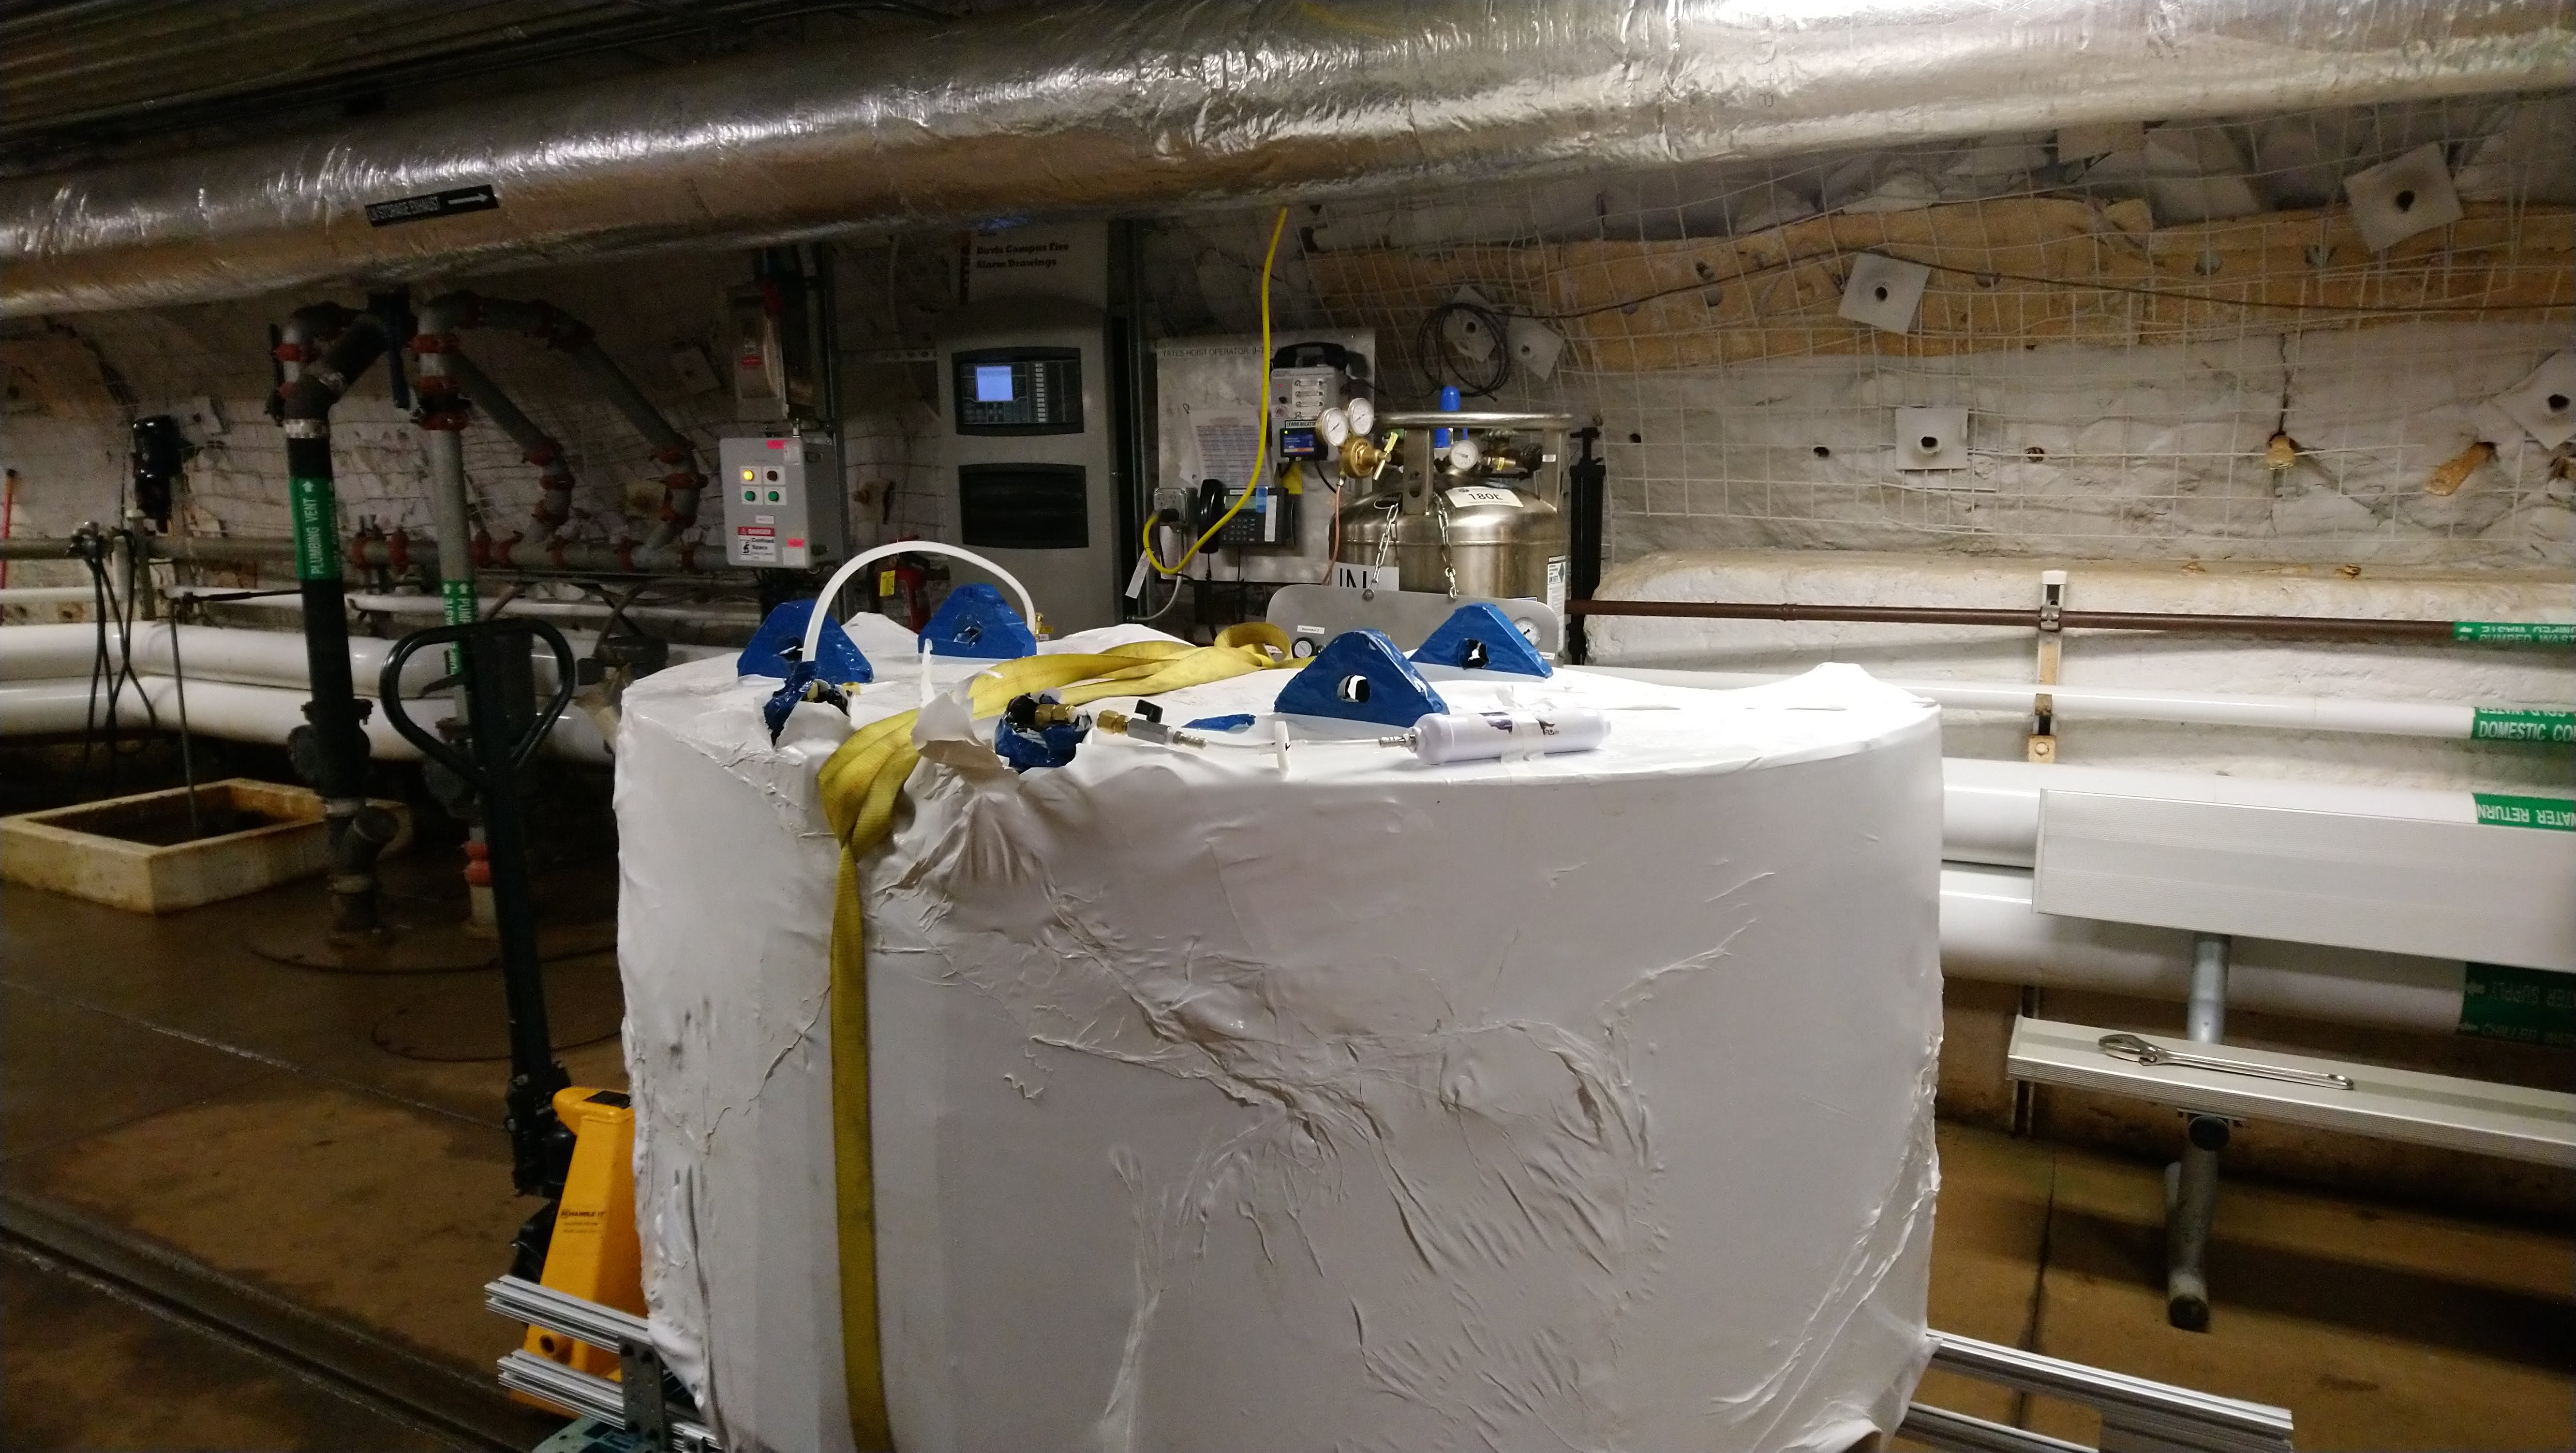
\includegraphics[width=\textwidth]{Figures/Construction/tat_purging.JPG}
\centering
\caption{Photograph of the a top tank setup for N2 purge.}
\label{fig:TAT_purging}
\end{figure}

\par
The proposed solution was to 'correct the curvature' with additional foam on top of the OCV, which due to construction delays and COVID-19, did not begin until August 2020.
The foam installed on the top of the OCV was of the same type as planned for the side tanks and assayed in \cite{LZ_assay_ref}.
The primary bonding methods used to secure the foam to the OCV was HandiFoam\textsuperscript{\textregistered} \cite{handifoam_ref}.
HandiFoam\textsuperscript{\textregistered} was chosen as it securely held test pieces together, but also would will in any potential gaps.
Additionally, the foam was held in place with titanium pins, and titanium rods.
Part of the installation is shown in Figure \ref{fig:TAT_foam_installation}.

\begin{figure}[!htbp]
\begin{subfigure}{.5\textwidth}
  \centering
  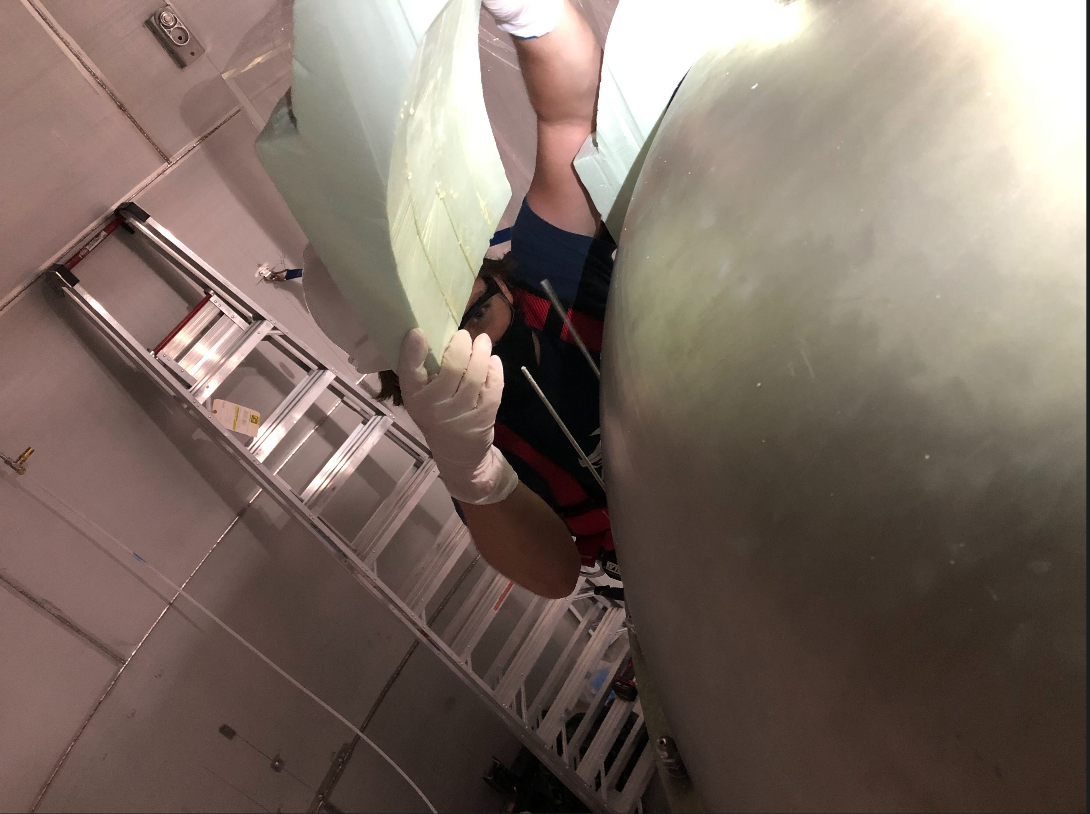
\includegraphics[width=\linewidth]{Figures/Construction/TAT_foam_installation.png}
  \end{subfigure}
  \begin{subfigure}{.5\textwidth}
  \centering
  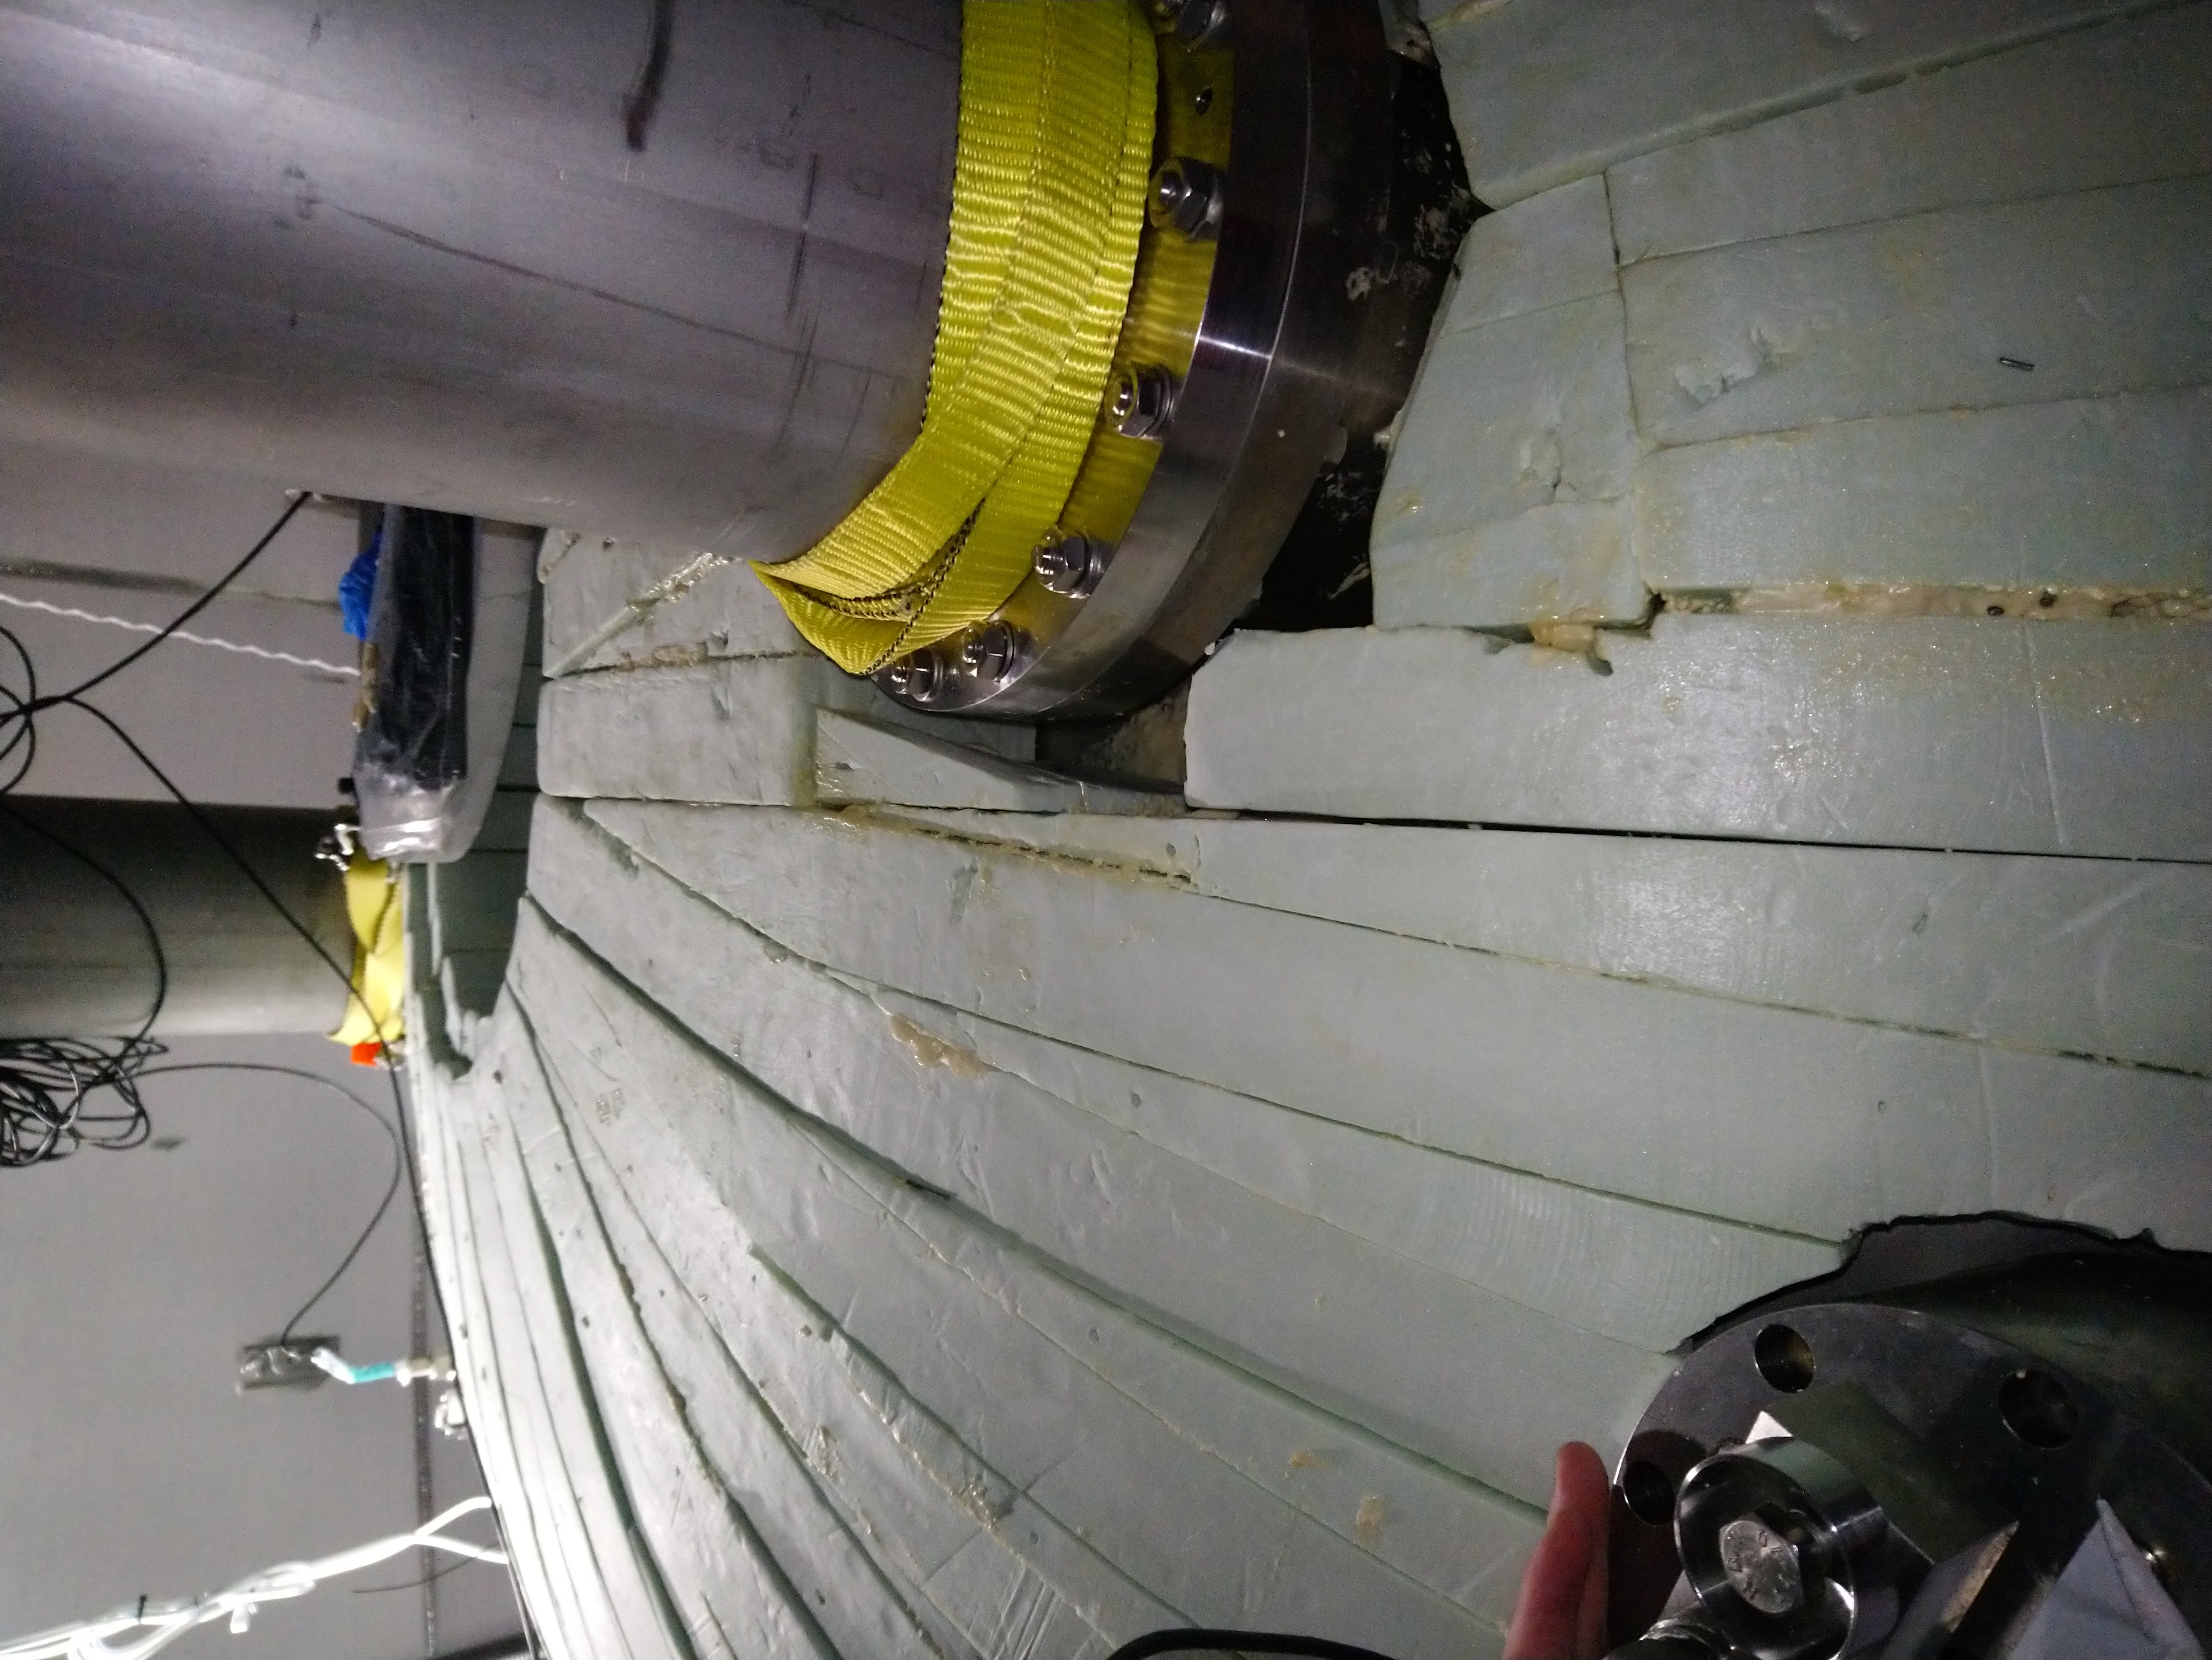
\includegraphics[angle=-90, width=\linewidth]{Figures/Construction/TAT_foam_complete.jpg}
  \end{subfigure}
\caption{Photograph of TAT-OCV foam installation.}
\label{fig:TAT_foam_installation}
\end{figure}

\par
The SAT-OCV foam was installed after the TAT-OCV foam in a slightly different fashion.
These pieces were primarily secured together using silicon sealant \cite{dowsil_silicone_ref} to each other and the OCV.
Titanium pins were also used to secure pieces together and trapping them behind the bolts on the OCV.
The final fit-test is shown in Figure \ref{fig:SAT_foam_guys}.

\par
As the foam had been underground for a number of weeks prior to being used, each piece of foam installed underwent a final 'shaving', shown in Figure \ref{fig:foam_saving}.
A few mm was taken from each side of the foam to remove Radon chain particles that may have embedded themselves in the foam.

\begin{figure}[!htbp]
  \begin{subfigure}{.5\textwidth}
  \centering
  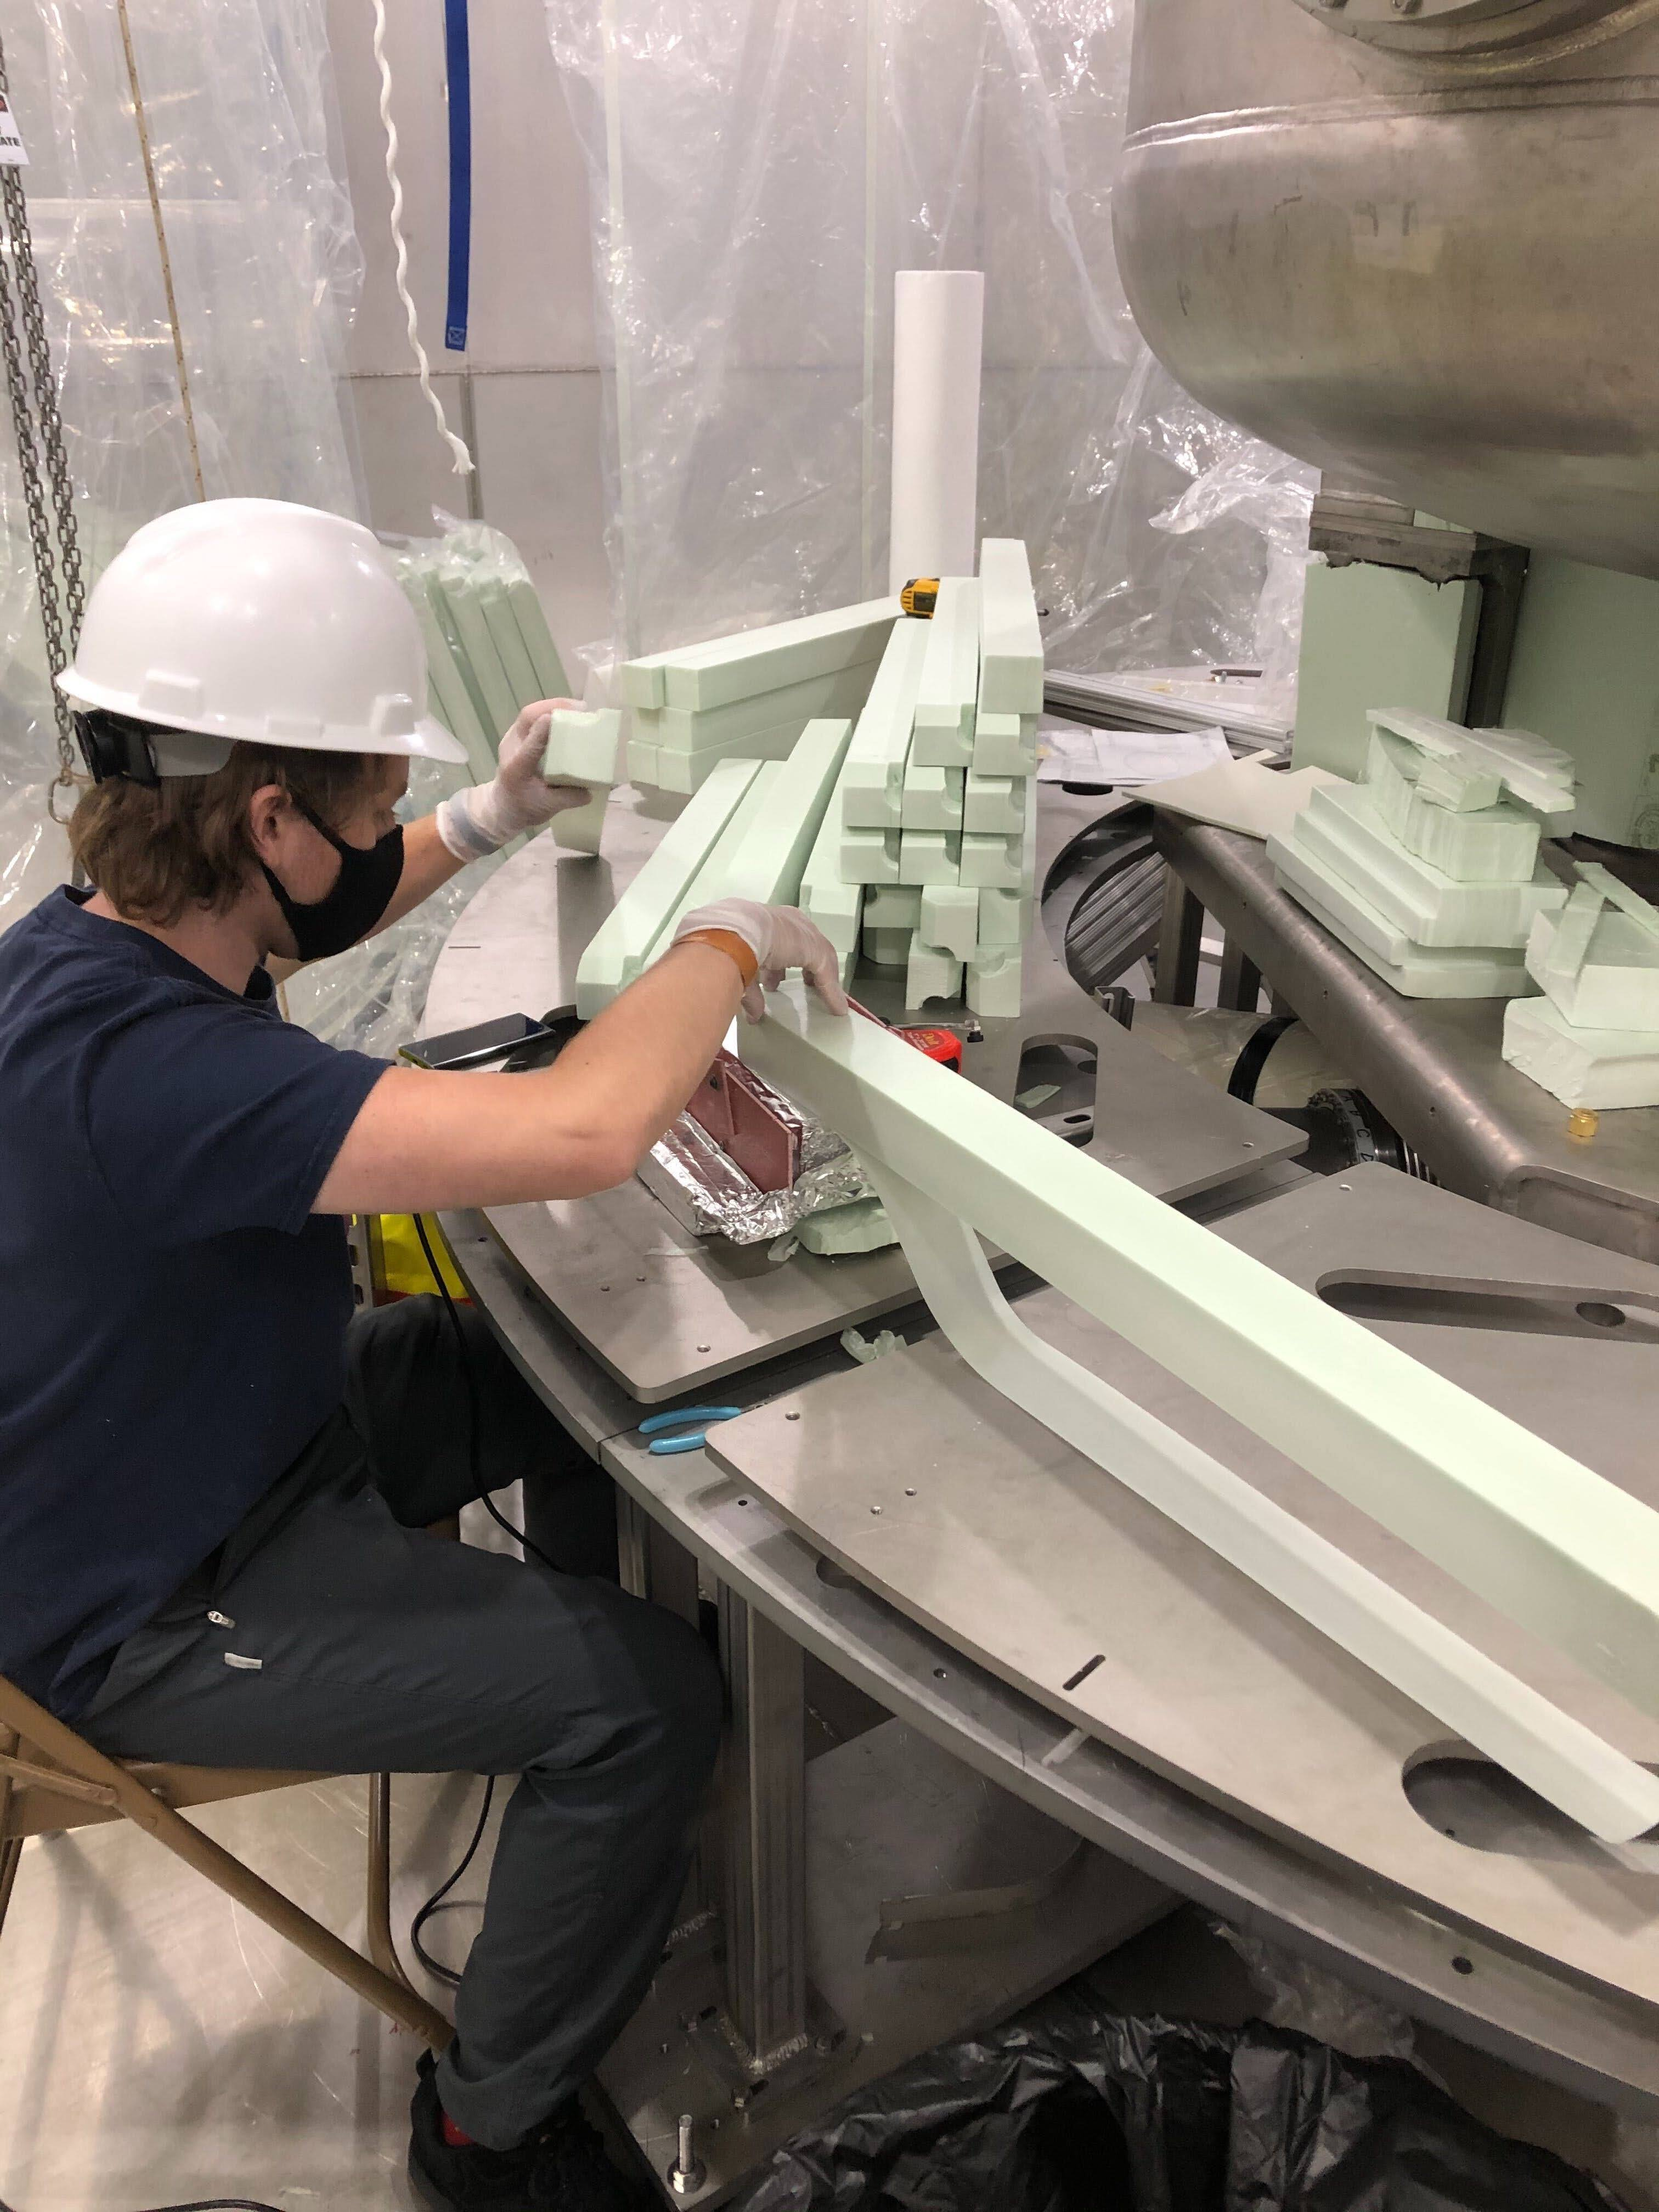
\includegraphics[width=\linewidth]{Figures/Construction/foam_shaving.jpg}
  \caption{Author using a hot-knife to shave all SAT foam prior to installation.}
  \label{fig:foam_saving}
  \end{subfigure}
  \begin{subfigure}{.5\textwidth}
  \centering
  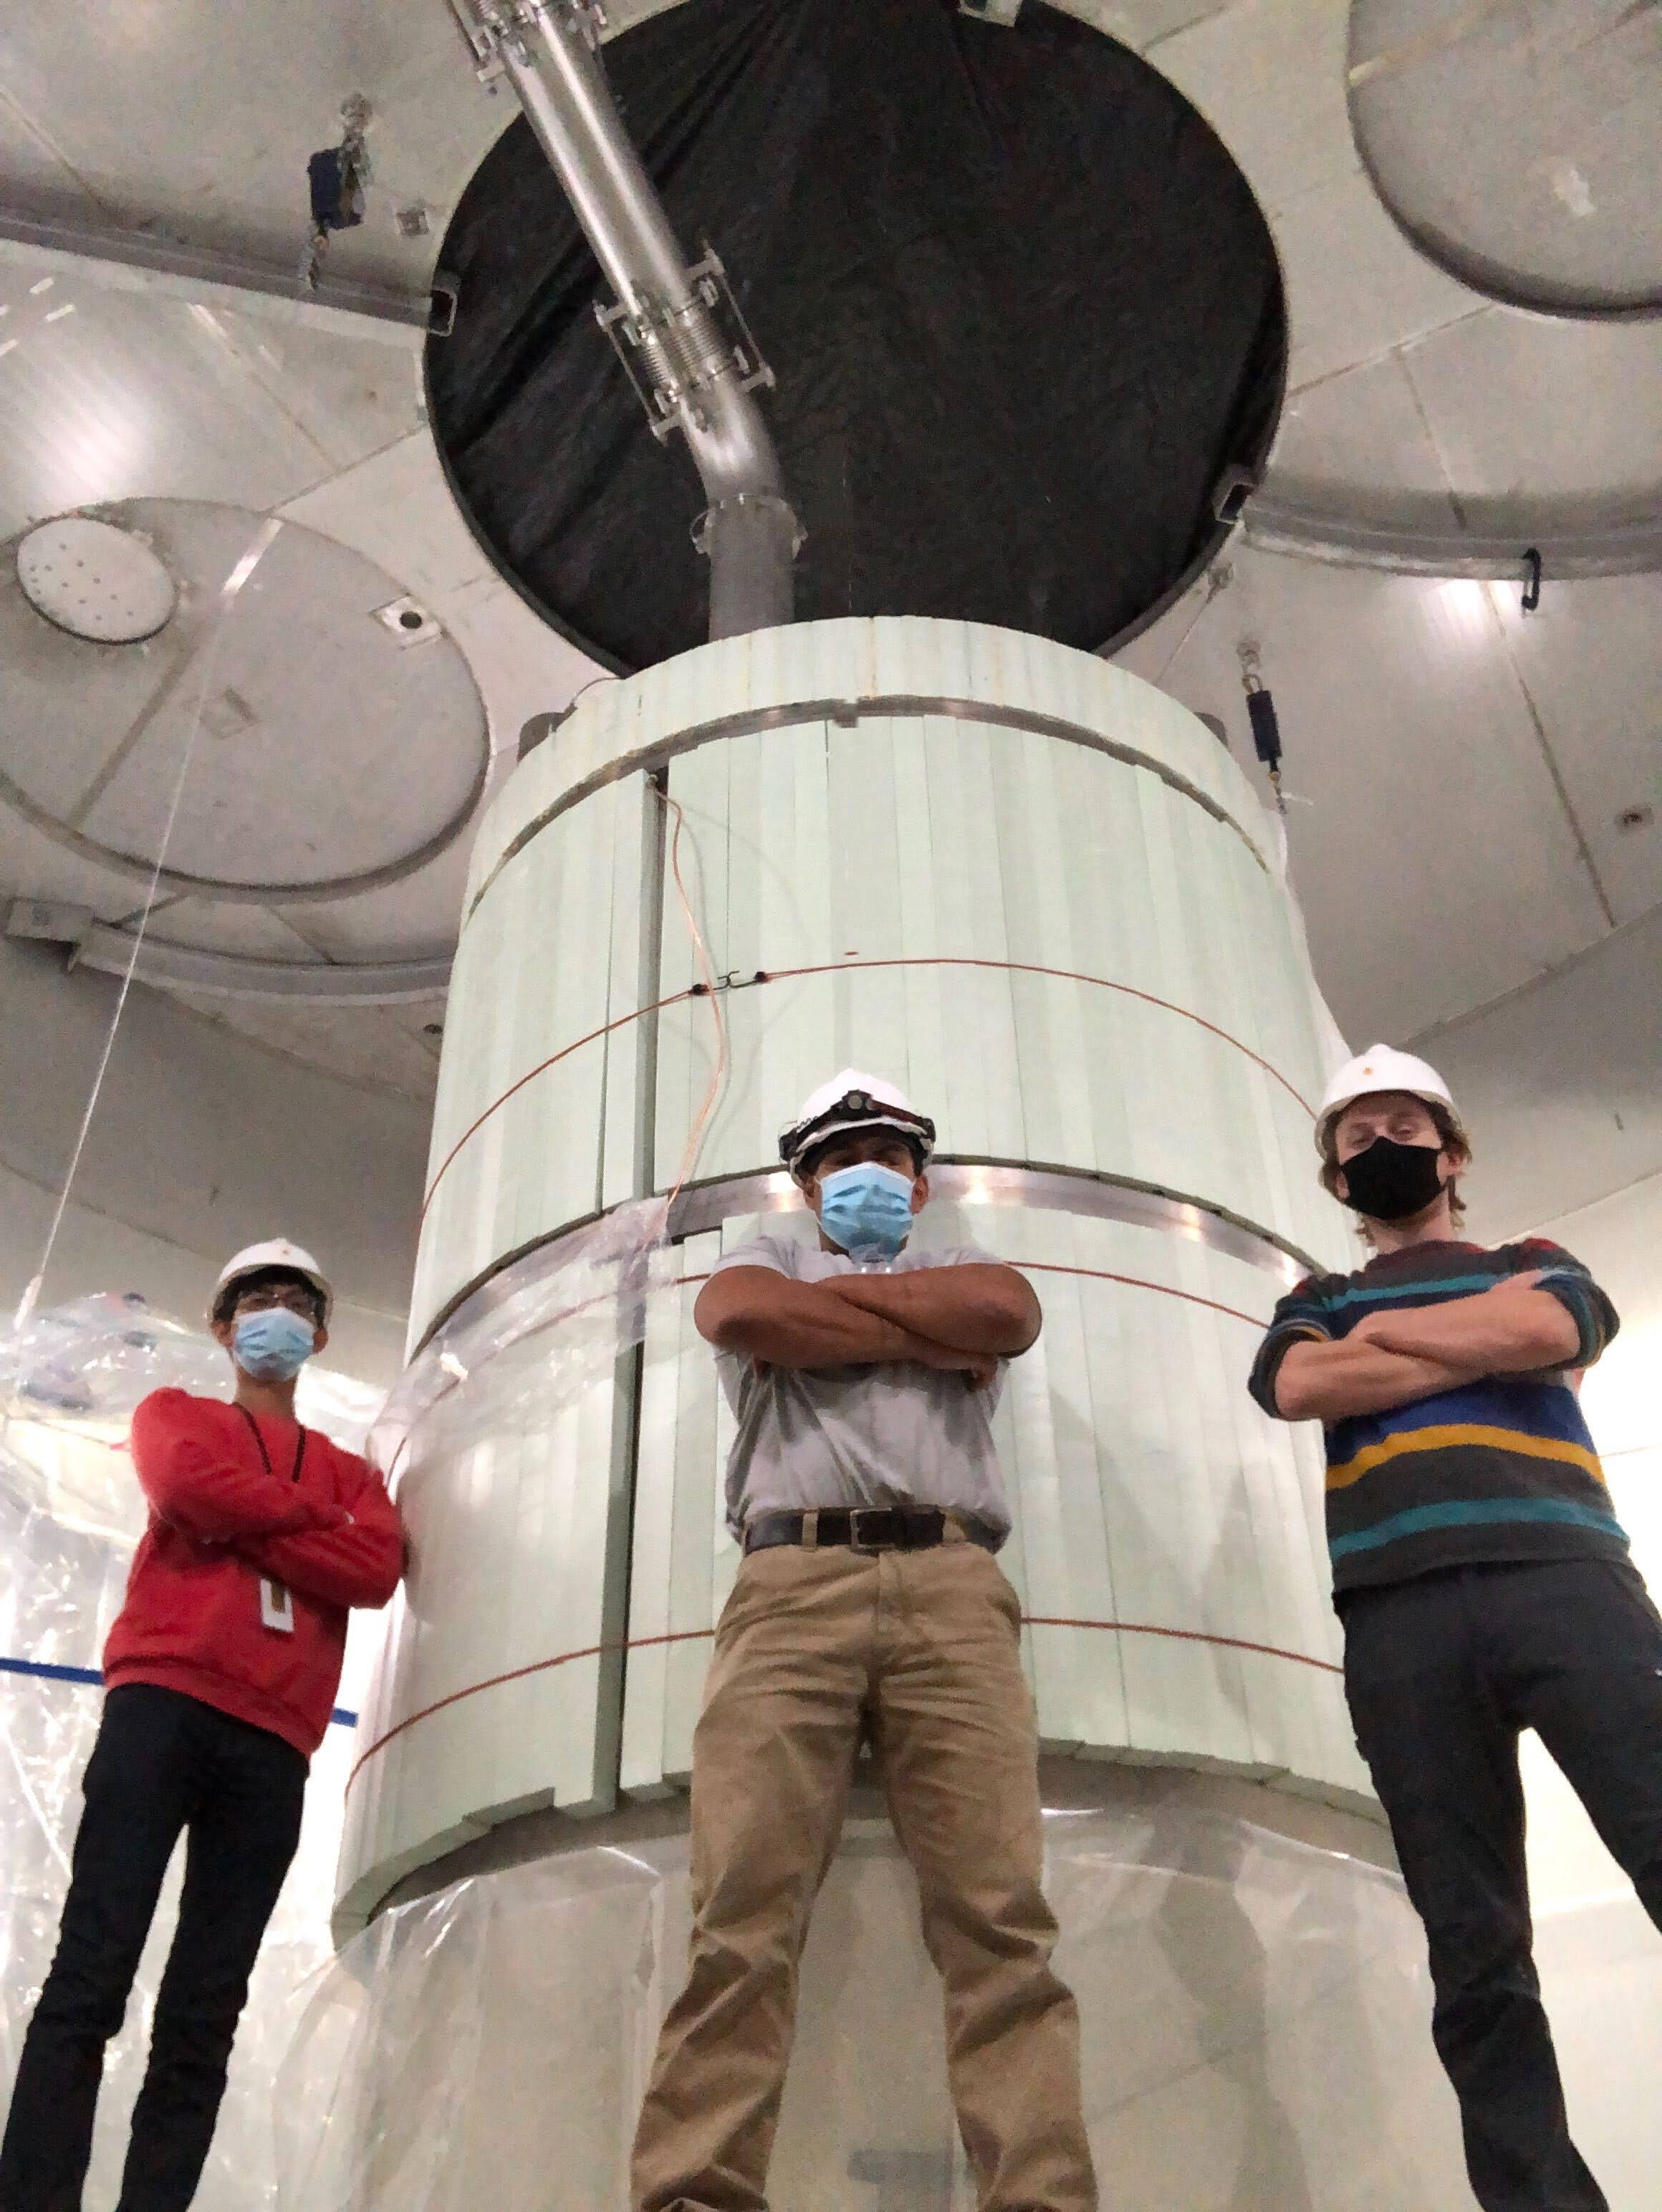
\includegraphics[width=\linewidth]{Figures/Construction/SAT_foam_fittest.jpg}
  \caption{OD installers Left to Right: Ryan Wang, Derek Lucero, Sam Eriksen}
  \label{fig:SAT_foam_guys}
  \end{subfigure}
\caption{Photographs of SAT-OCV foam installation.}
\label{fig:SAT_foam_installation}
\end{figure}

\par
Additional foam was installed around the OCV legs in between the BATs.
This foam was secured using HandiFoam\textsuperscript{\textregistered} as shown in Figure \ref{fig:ocv_leg_foam}.

\begin{figure}[!htbp]
\begin{subfigure}{.5\textwidth}
  \centering
  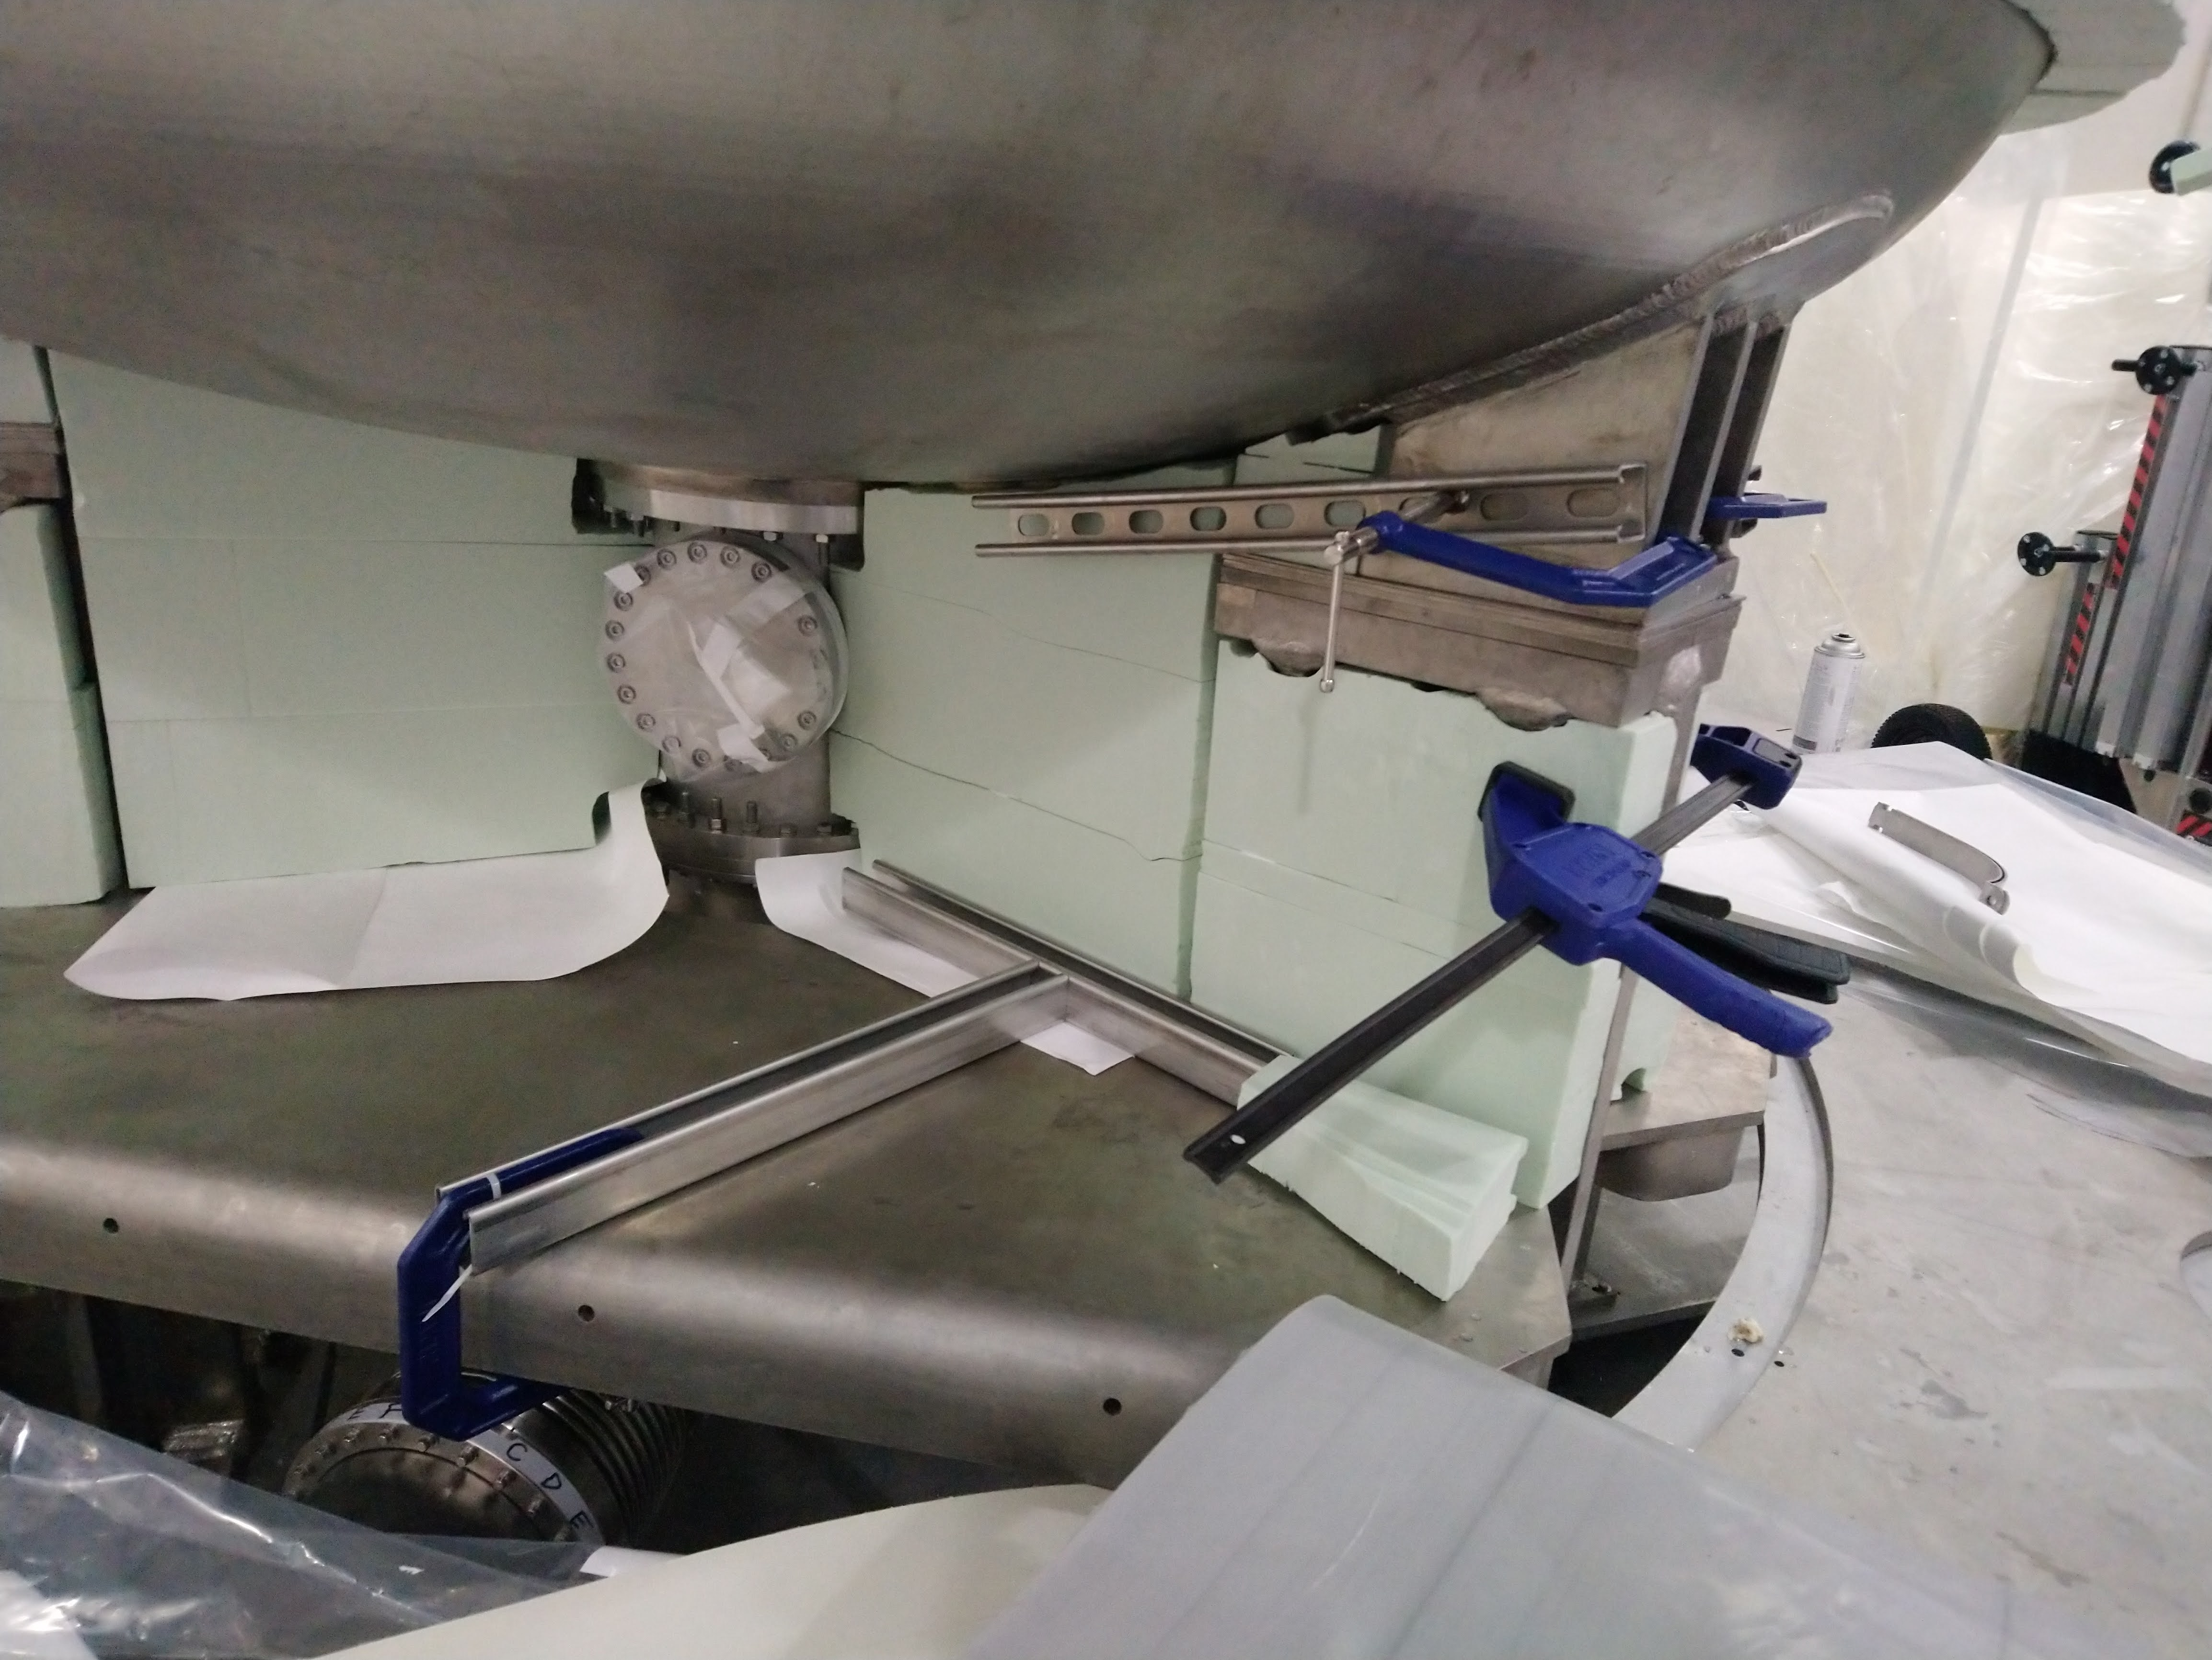
\includegraphics[height=5cm, width=\linewidth]{Figures/Construction/BAT_green_foam.JPG}
  \caption{OVV leg foam installation.}
  \label{fig:ocv_leg_foam}
  \end{subfigure}
  \begin{subfigure}{.5\textwidth}
  \centering
  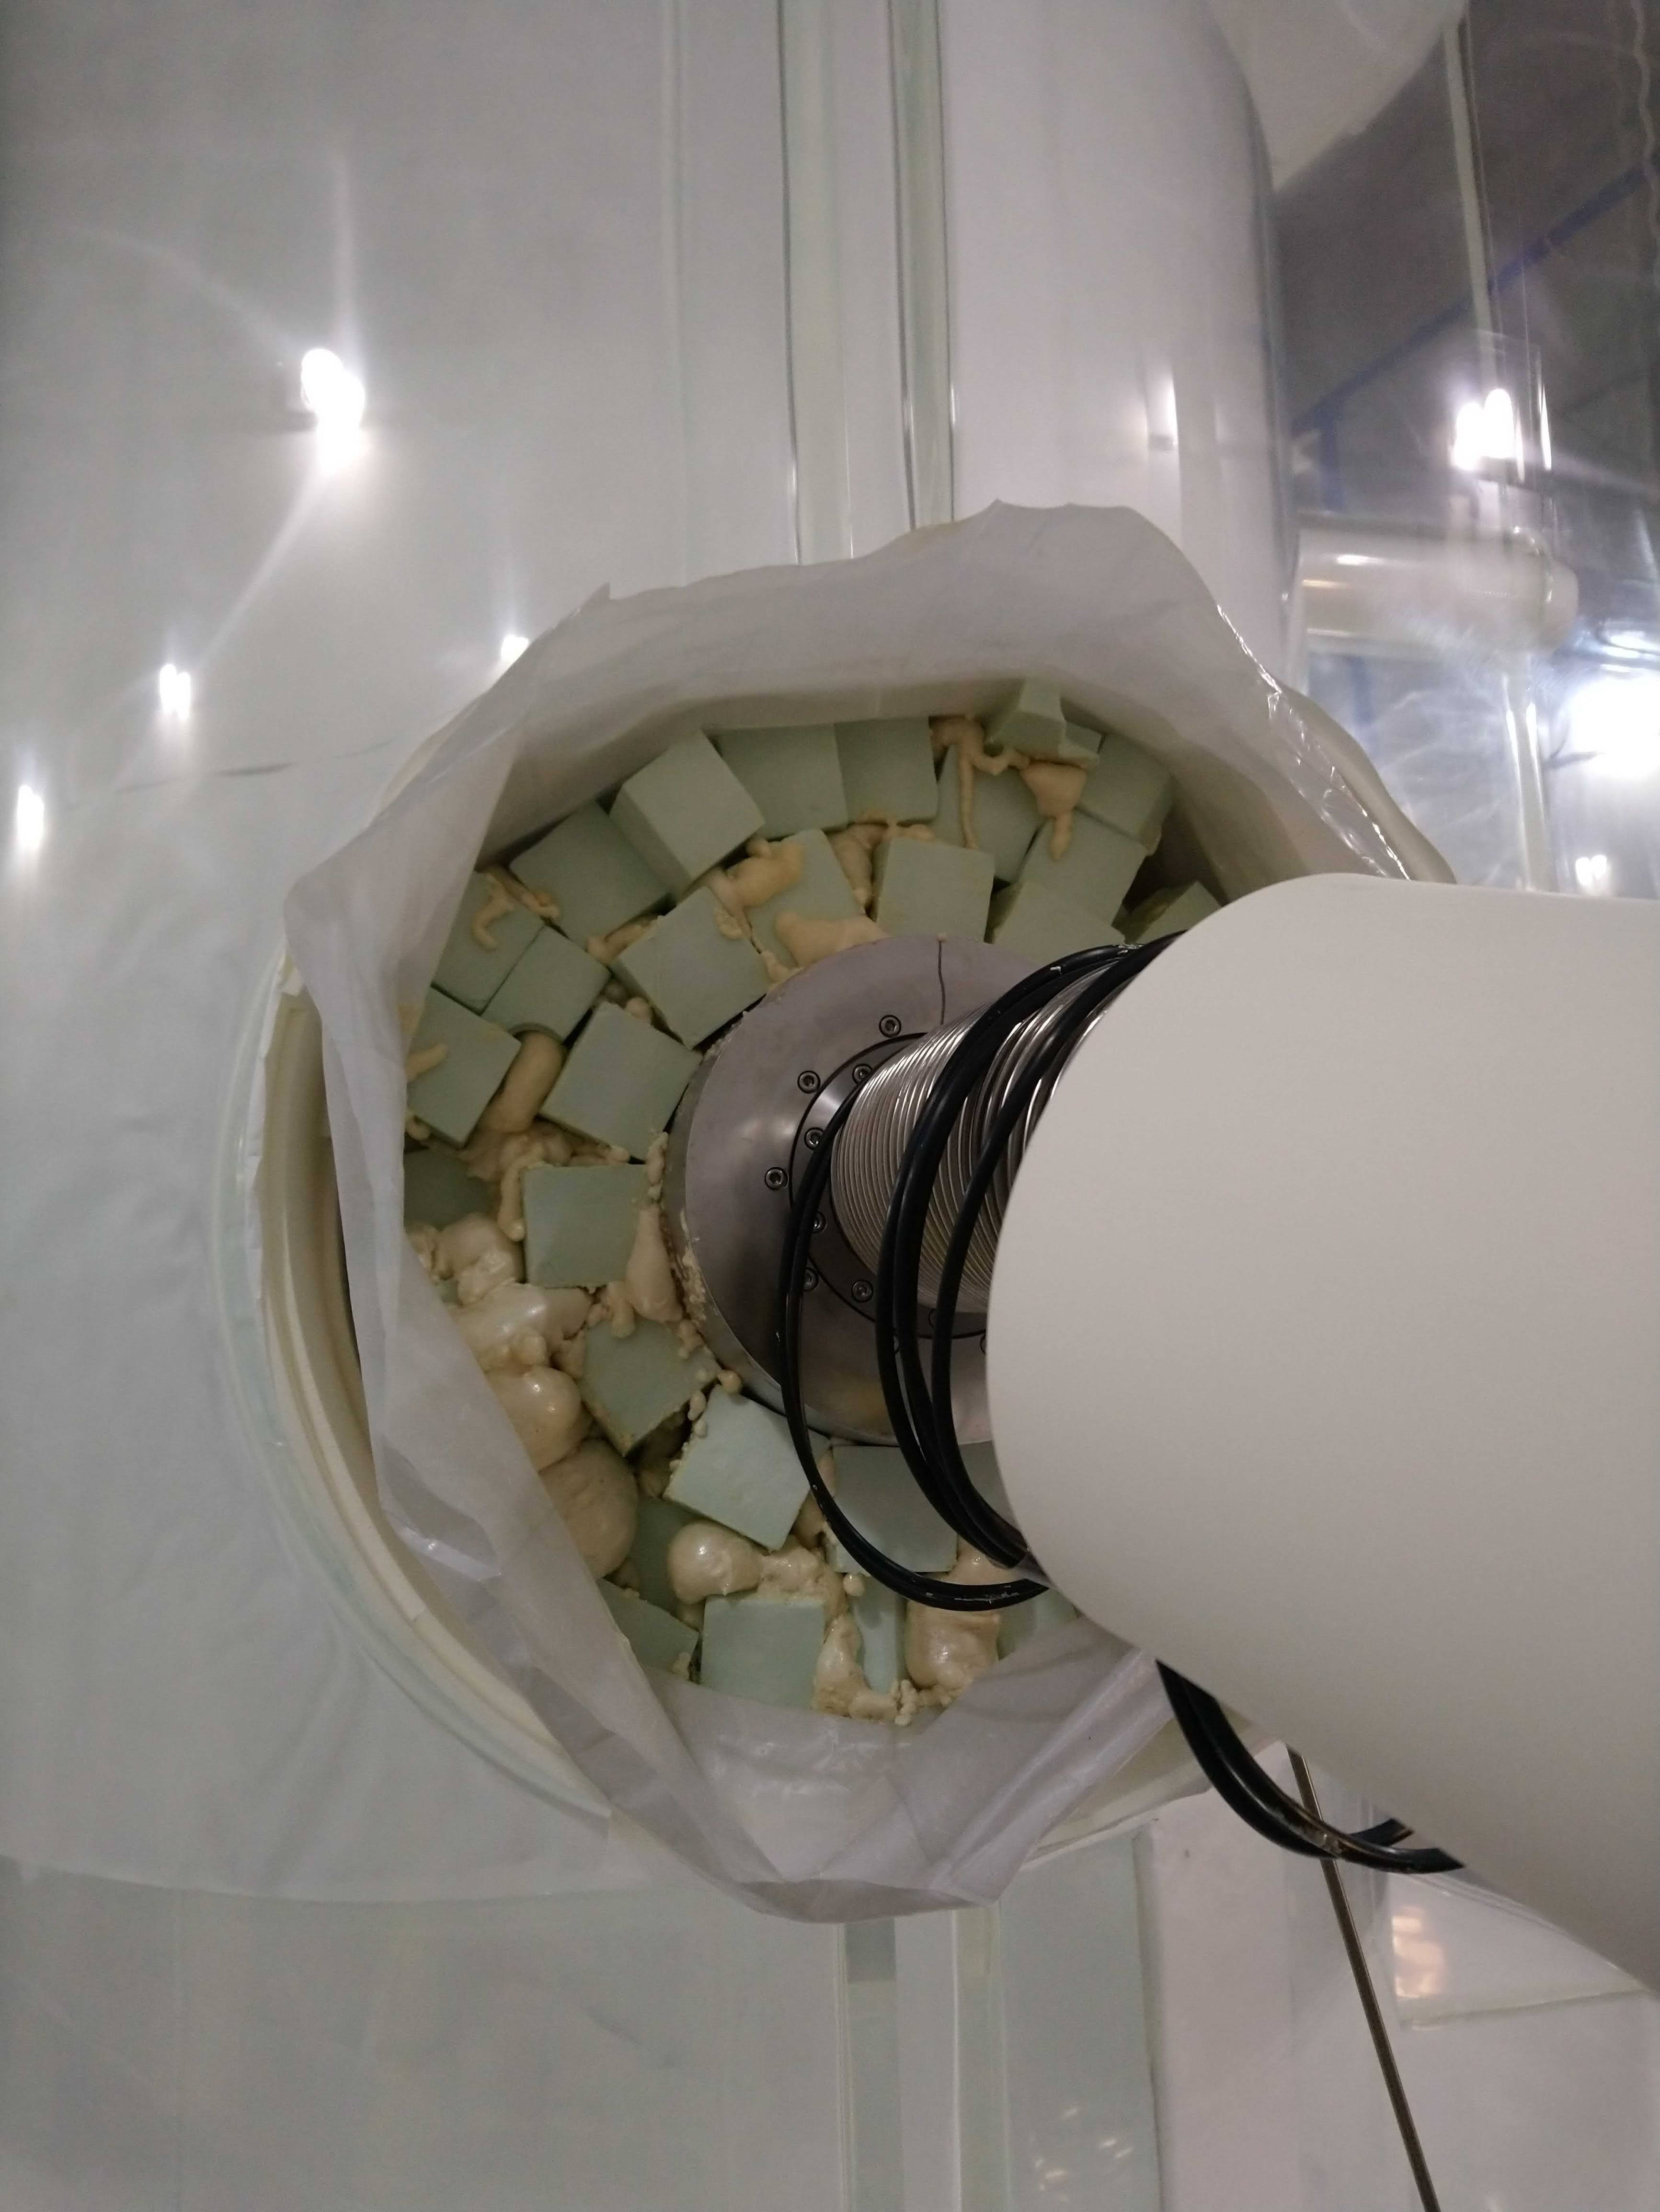
\includegraphics[height=5cm, width=\linewidth]{Figures/Construction/HV_foam.jpg}
  \caption{Foam installed around HV-feedthrough in SATs.}
  \label{fig:hv_port_foam}
  \end{subfigure}
\caption{Photographs of foam installed around OCV and HV-feedthrough.}
\label{fig:Additional_foam_installation}
\end{figure}

\par
Because of the aforementioned split tank and thin walls, there was a danger that the tanks may leak GdLS.
As the GdLS is oil-based it would float to the top of the water, however experiments showed that it did not react well with the foam surrounding the OCV.
As such, polyethylene sheets were installed to cover the foam. 
On top of this, the Tyvek was installed.
In addition, the OD-Tyvek shape around the TAT was changed.
Previously this was a flat Tyvek sheet lying on top of the TAT and out to the OD PMTs.
However, in order to allow for a potential GdLS leak to reach the surface, a TeePee design was adopted.


\par
During the BAT test-fitting, it was found that these also did not match the curvature of the OCV.
Additionally, because of the placement of the securing feet underneath them, they were not stable.
This mean that as the water tank was filled, the BATs would be able to rock and bash into the OCV and potentially break their feet off.
The installation solution was to secure the BATs as much as possible with foam.
A different, thinner foam was selected for this purpose as it was more flexible.
Additionally, HandiFoam\textsuperscript{\textregistered} was used for smaller places that could not be reached.
Neither of these foam solutions had been assayed.
The final BAT installation is shown in Figure \ref{fig:BAT_installation}.

\begin{figure}[!htbp]
\begin{subfigure}{.5\textwidth}
  \centering
  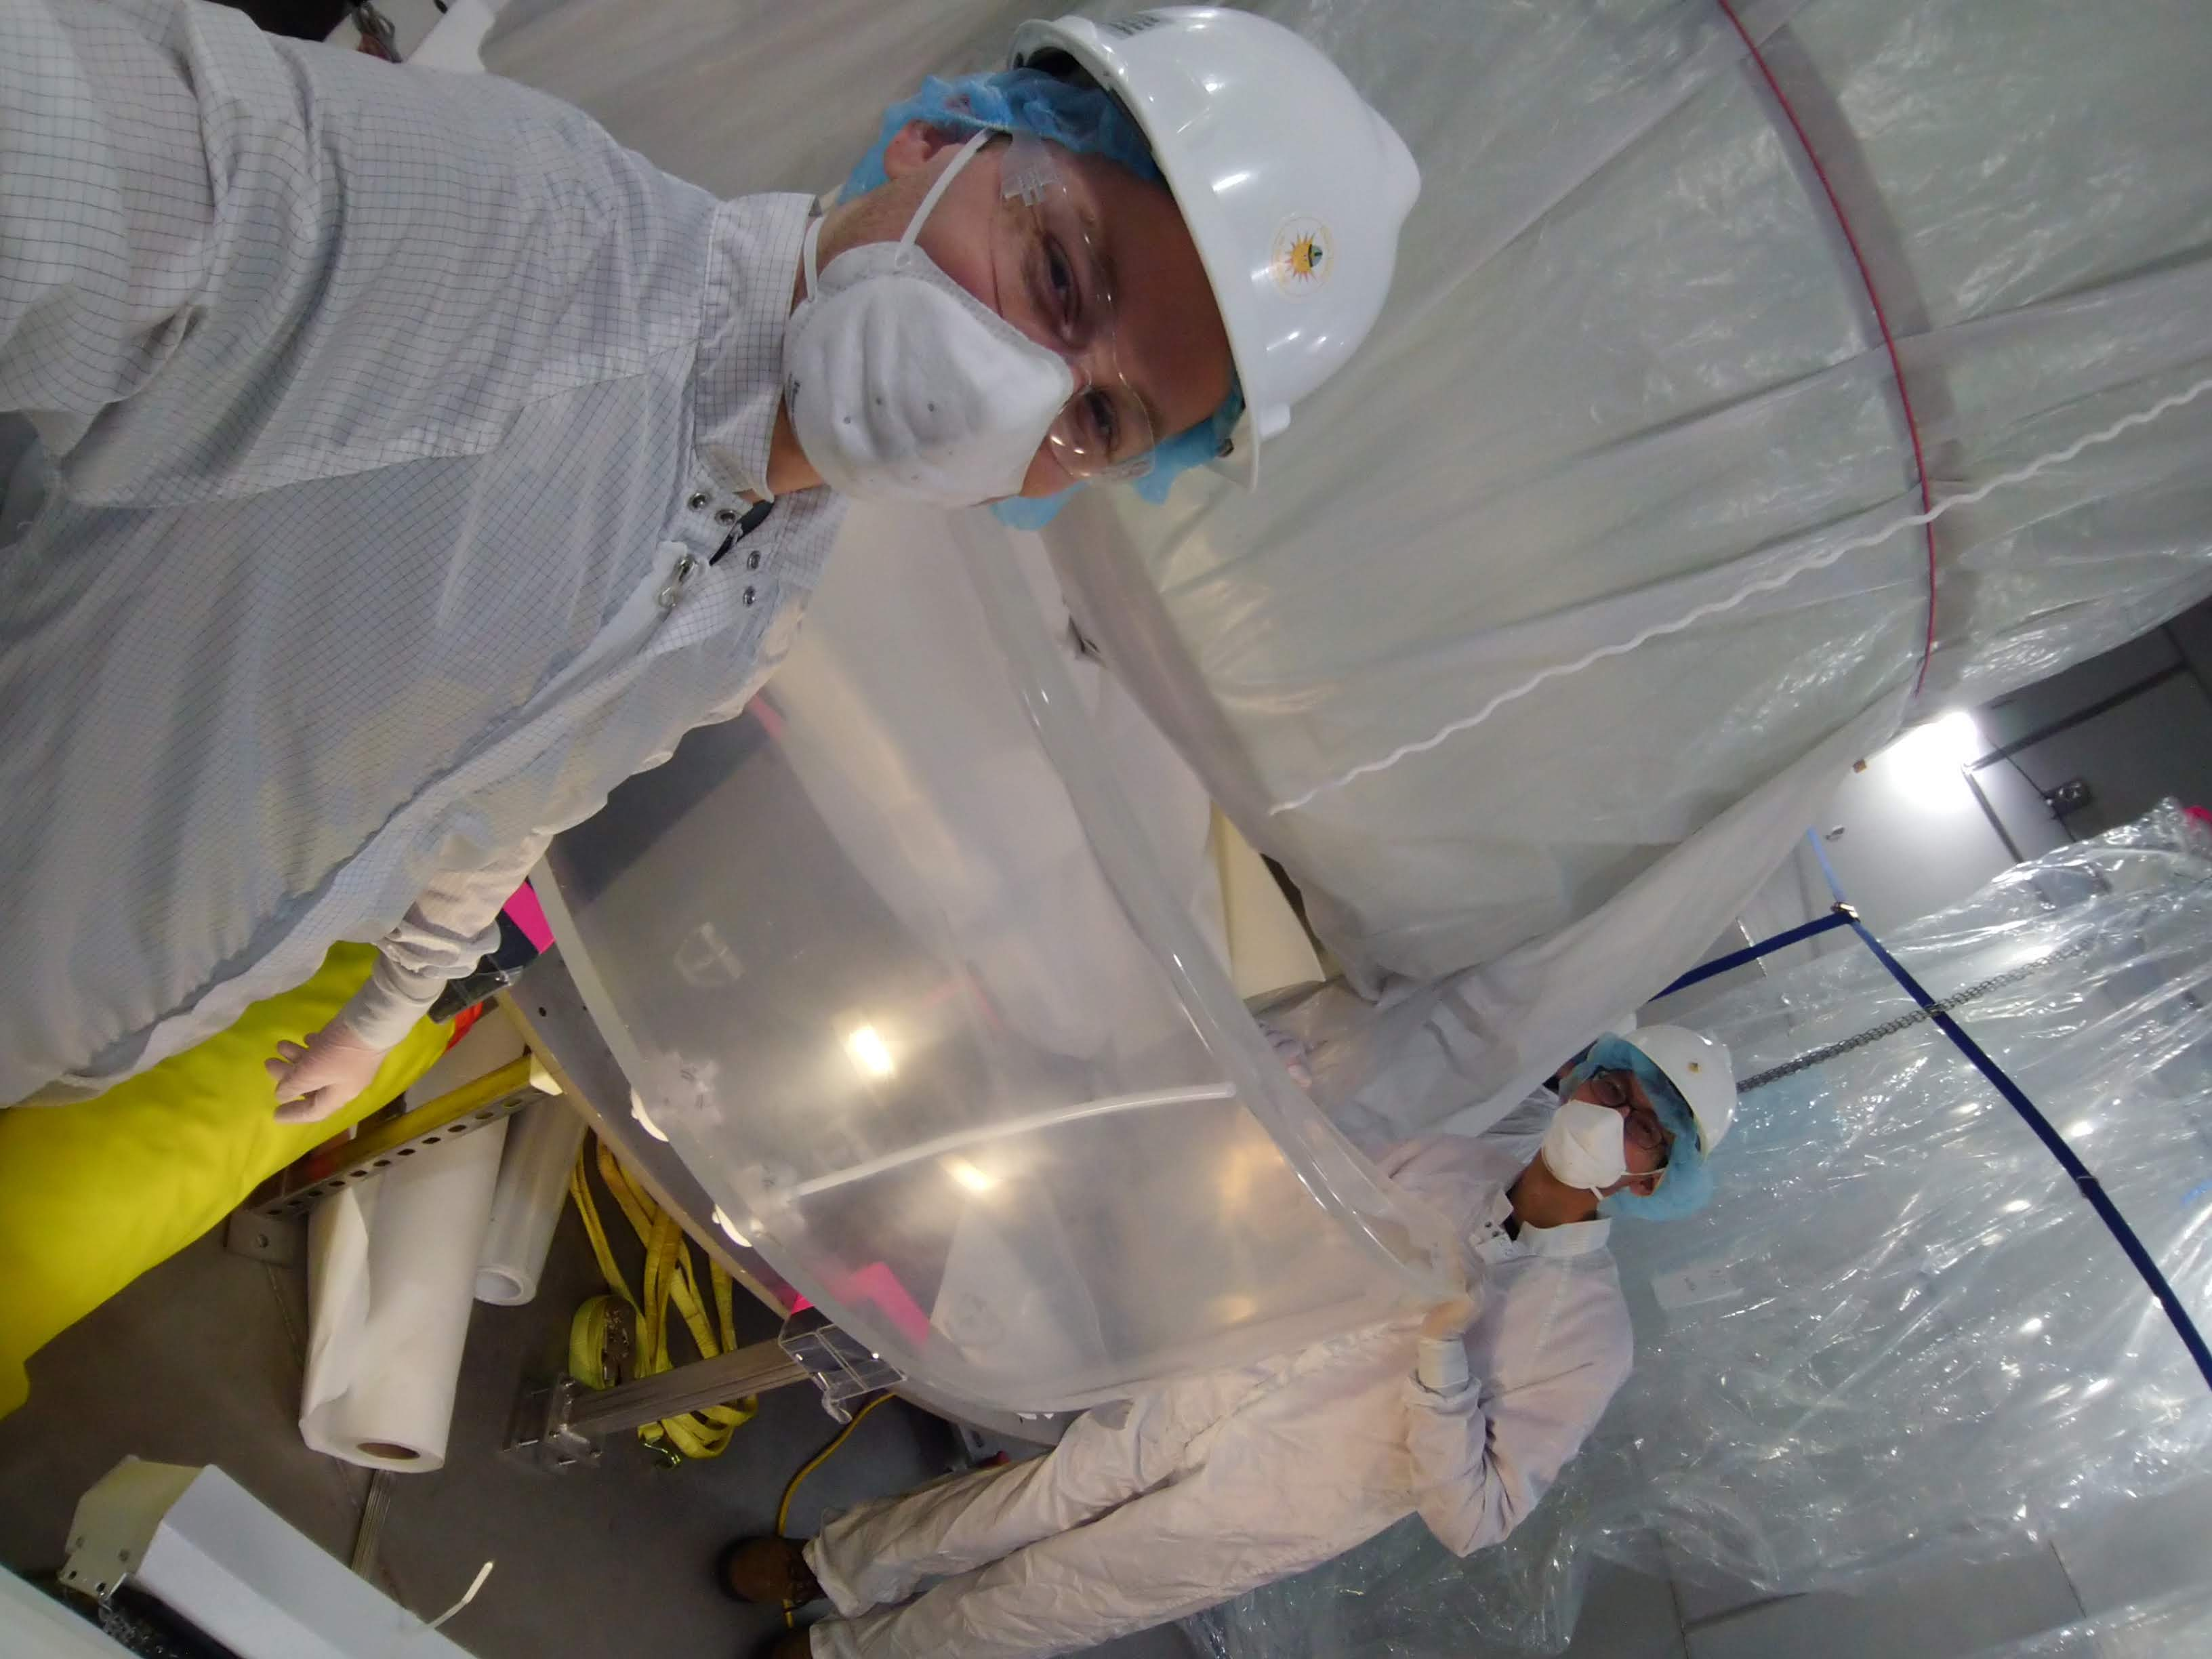
\includegraphics[angle=90, width=\linewidth]{Figures/Construction/BAT_installation.jpg}
  \caption{Installation of the final BAT}
  \label{fig:BAT_installation}
  \end{subfigure}
  \begin{subfigure}{.5\textwidth}
  \centering
  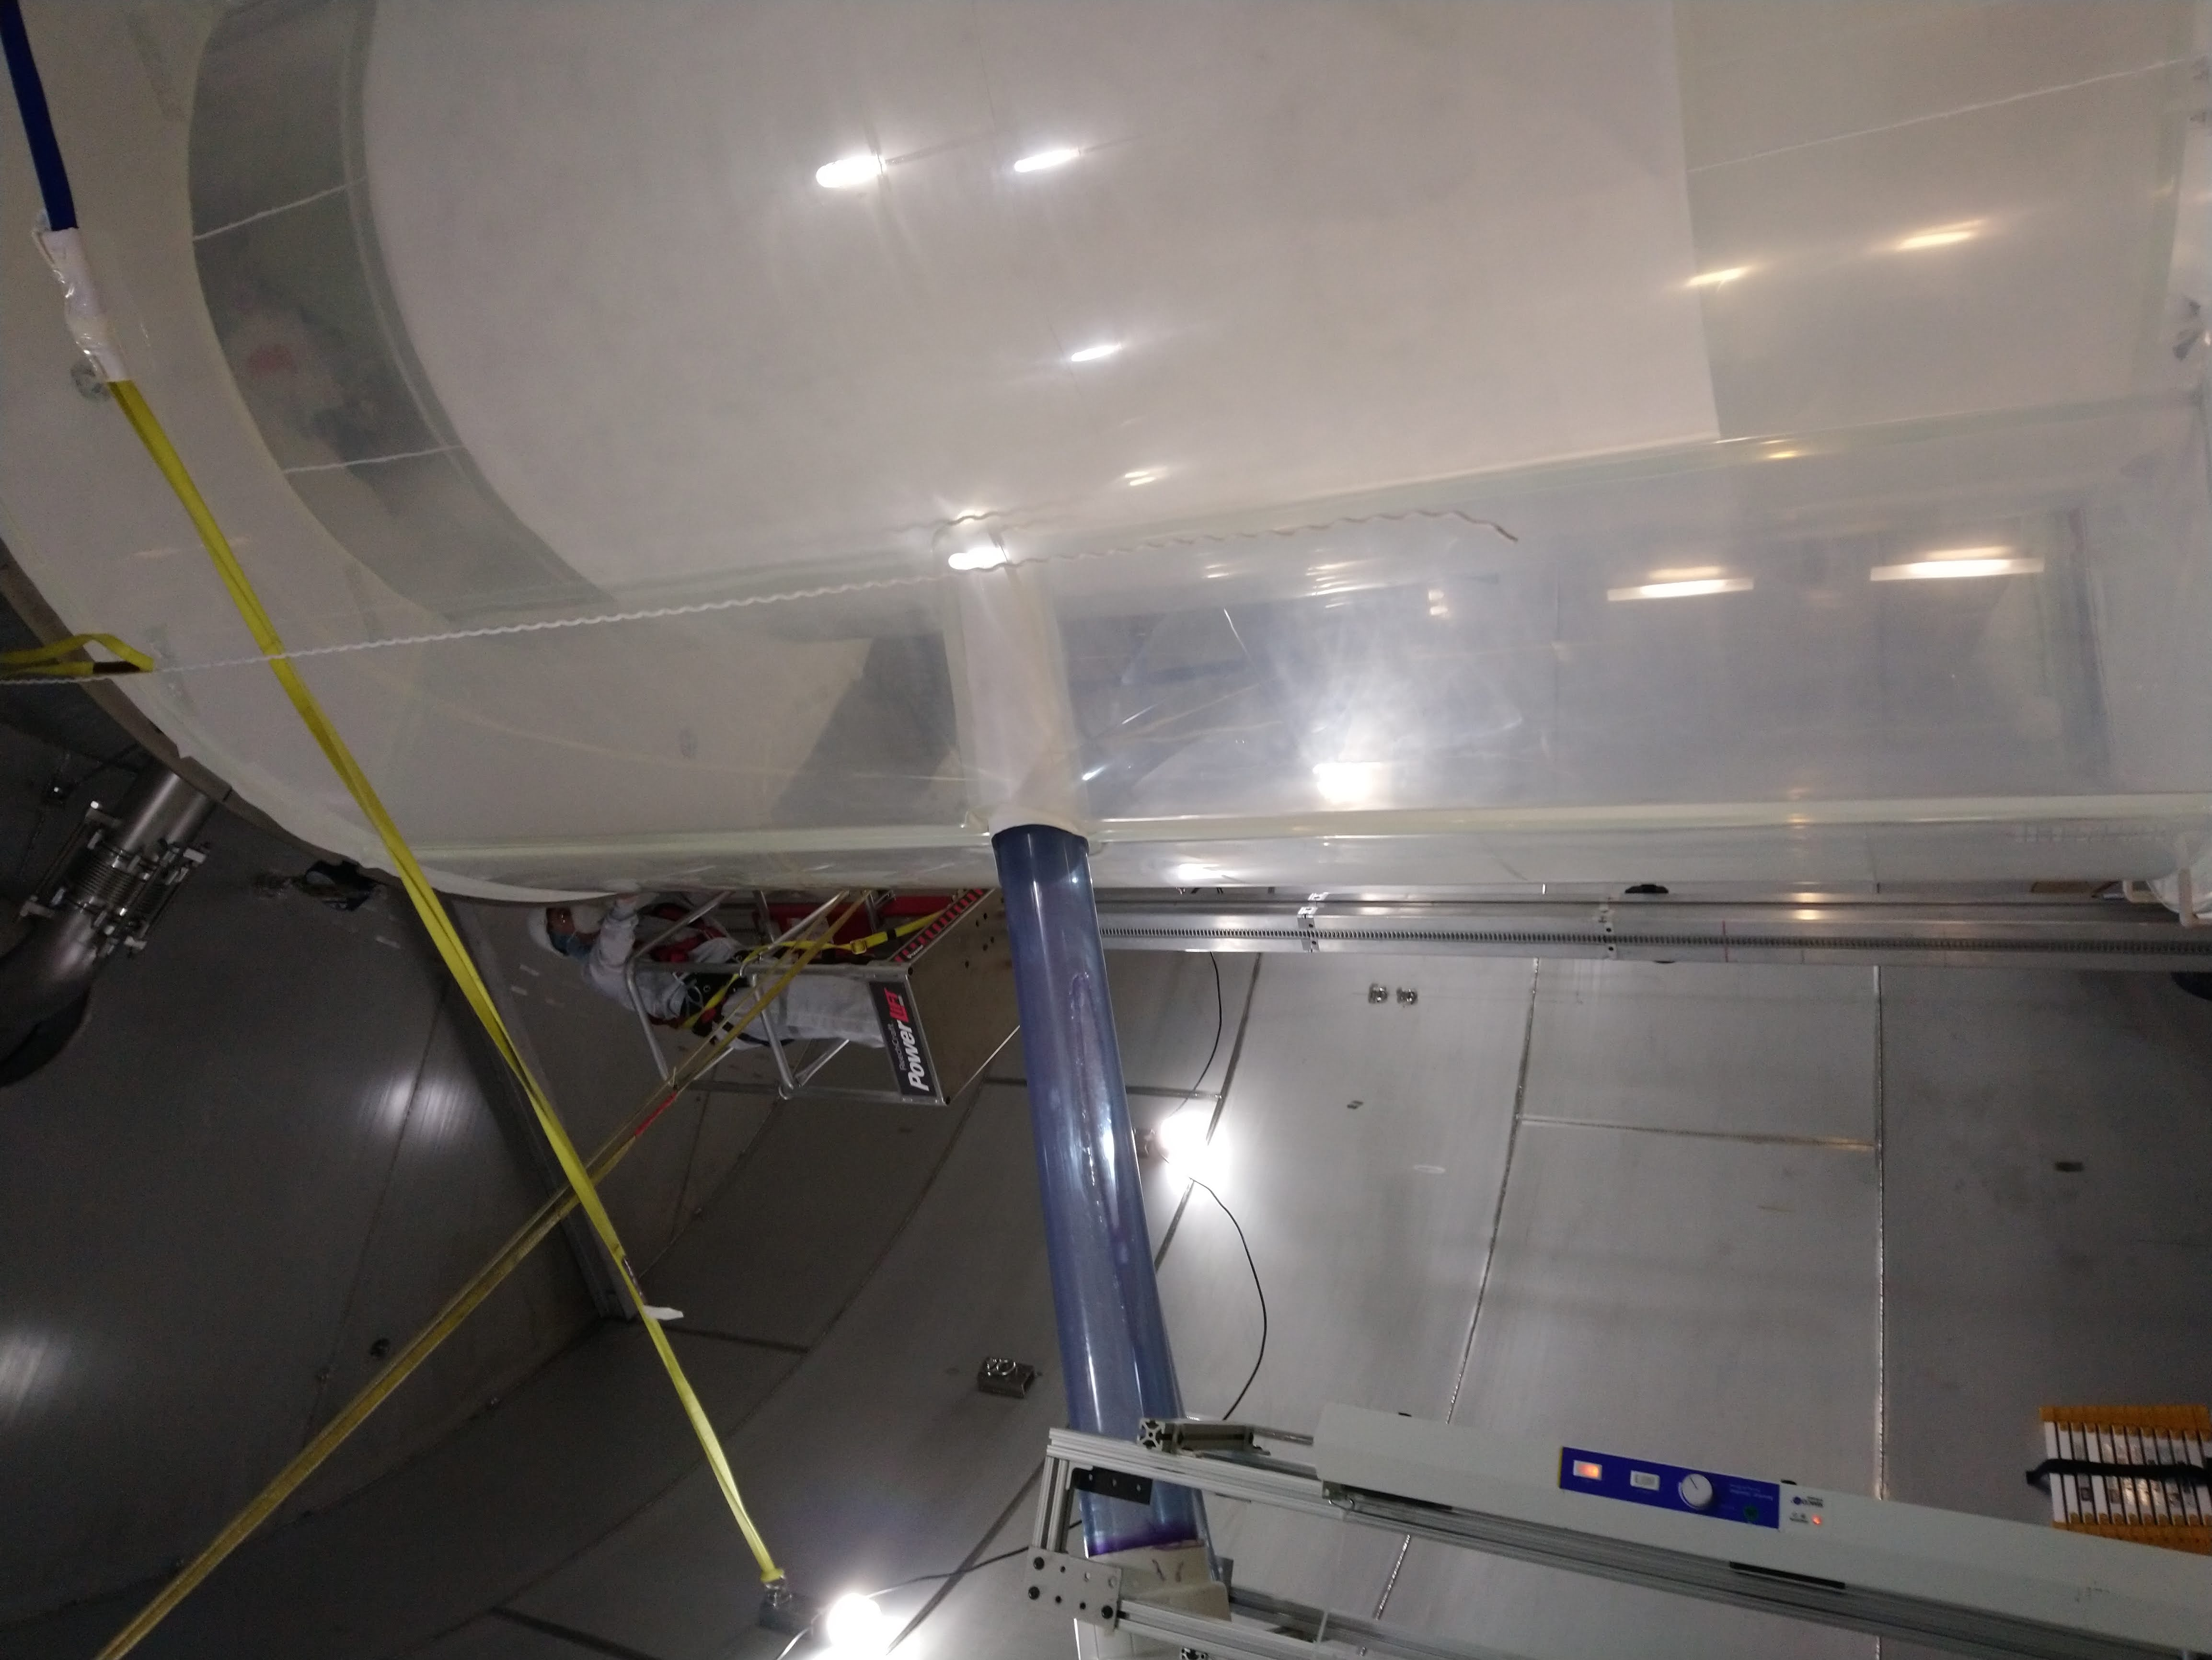
\includegraphics[angle=-90, width=\linewidth]{Figures/Construction/SAT_titanium_plate.JPG}
  \caption{Author securing the SAT.}
  \label{fig:SAT_titanium_installation}
  \end{subfigure}
\caption{Photographs of BAT and BAT installation.}
\label{fig:sat_and_bat_installation}
\end{figure}

\par
In additional to what has been mentioned, the SATs were secured using titanium plates.
To even the load the SATs experiences, 1-inch thick foam was installed above and below.
Additional foam was installed and secured with HandiFoam\textsuperscript{\textregistered} around the High Voltage port, where previously this was just water.
This is shown in Figure \ref{fig:hv_port_foam}.

\par
The Tyvek was installed as single layers with excess overlapping.
The use of a single layer will have a performance reduction with the reflectivity reducing by $\approx$10\% compared to multiple layers bonded together \cite{tyvek_reflectivity_ref}.

\par
The culmination of this is the completed OD, shown in Figure \ref{fig:complete_od}.

\begin{figure}[!htbp]
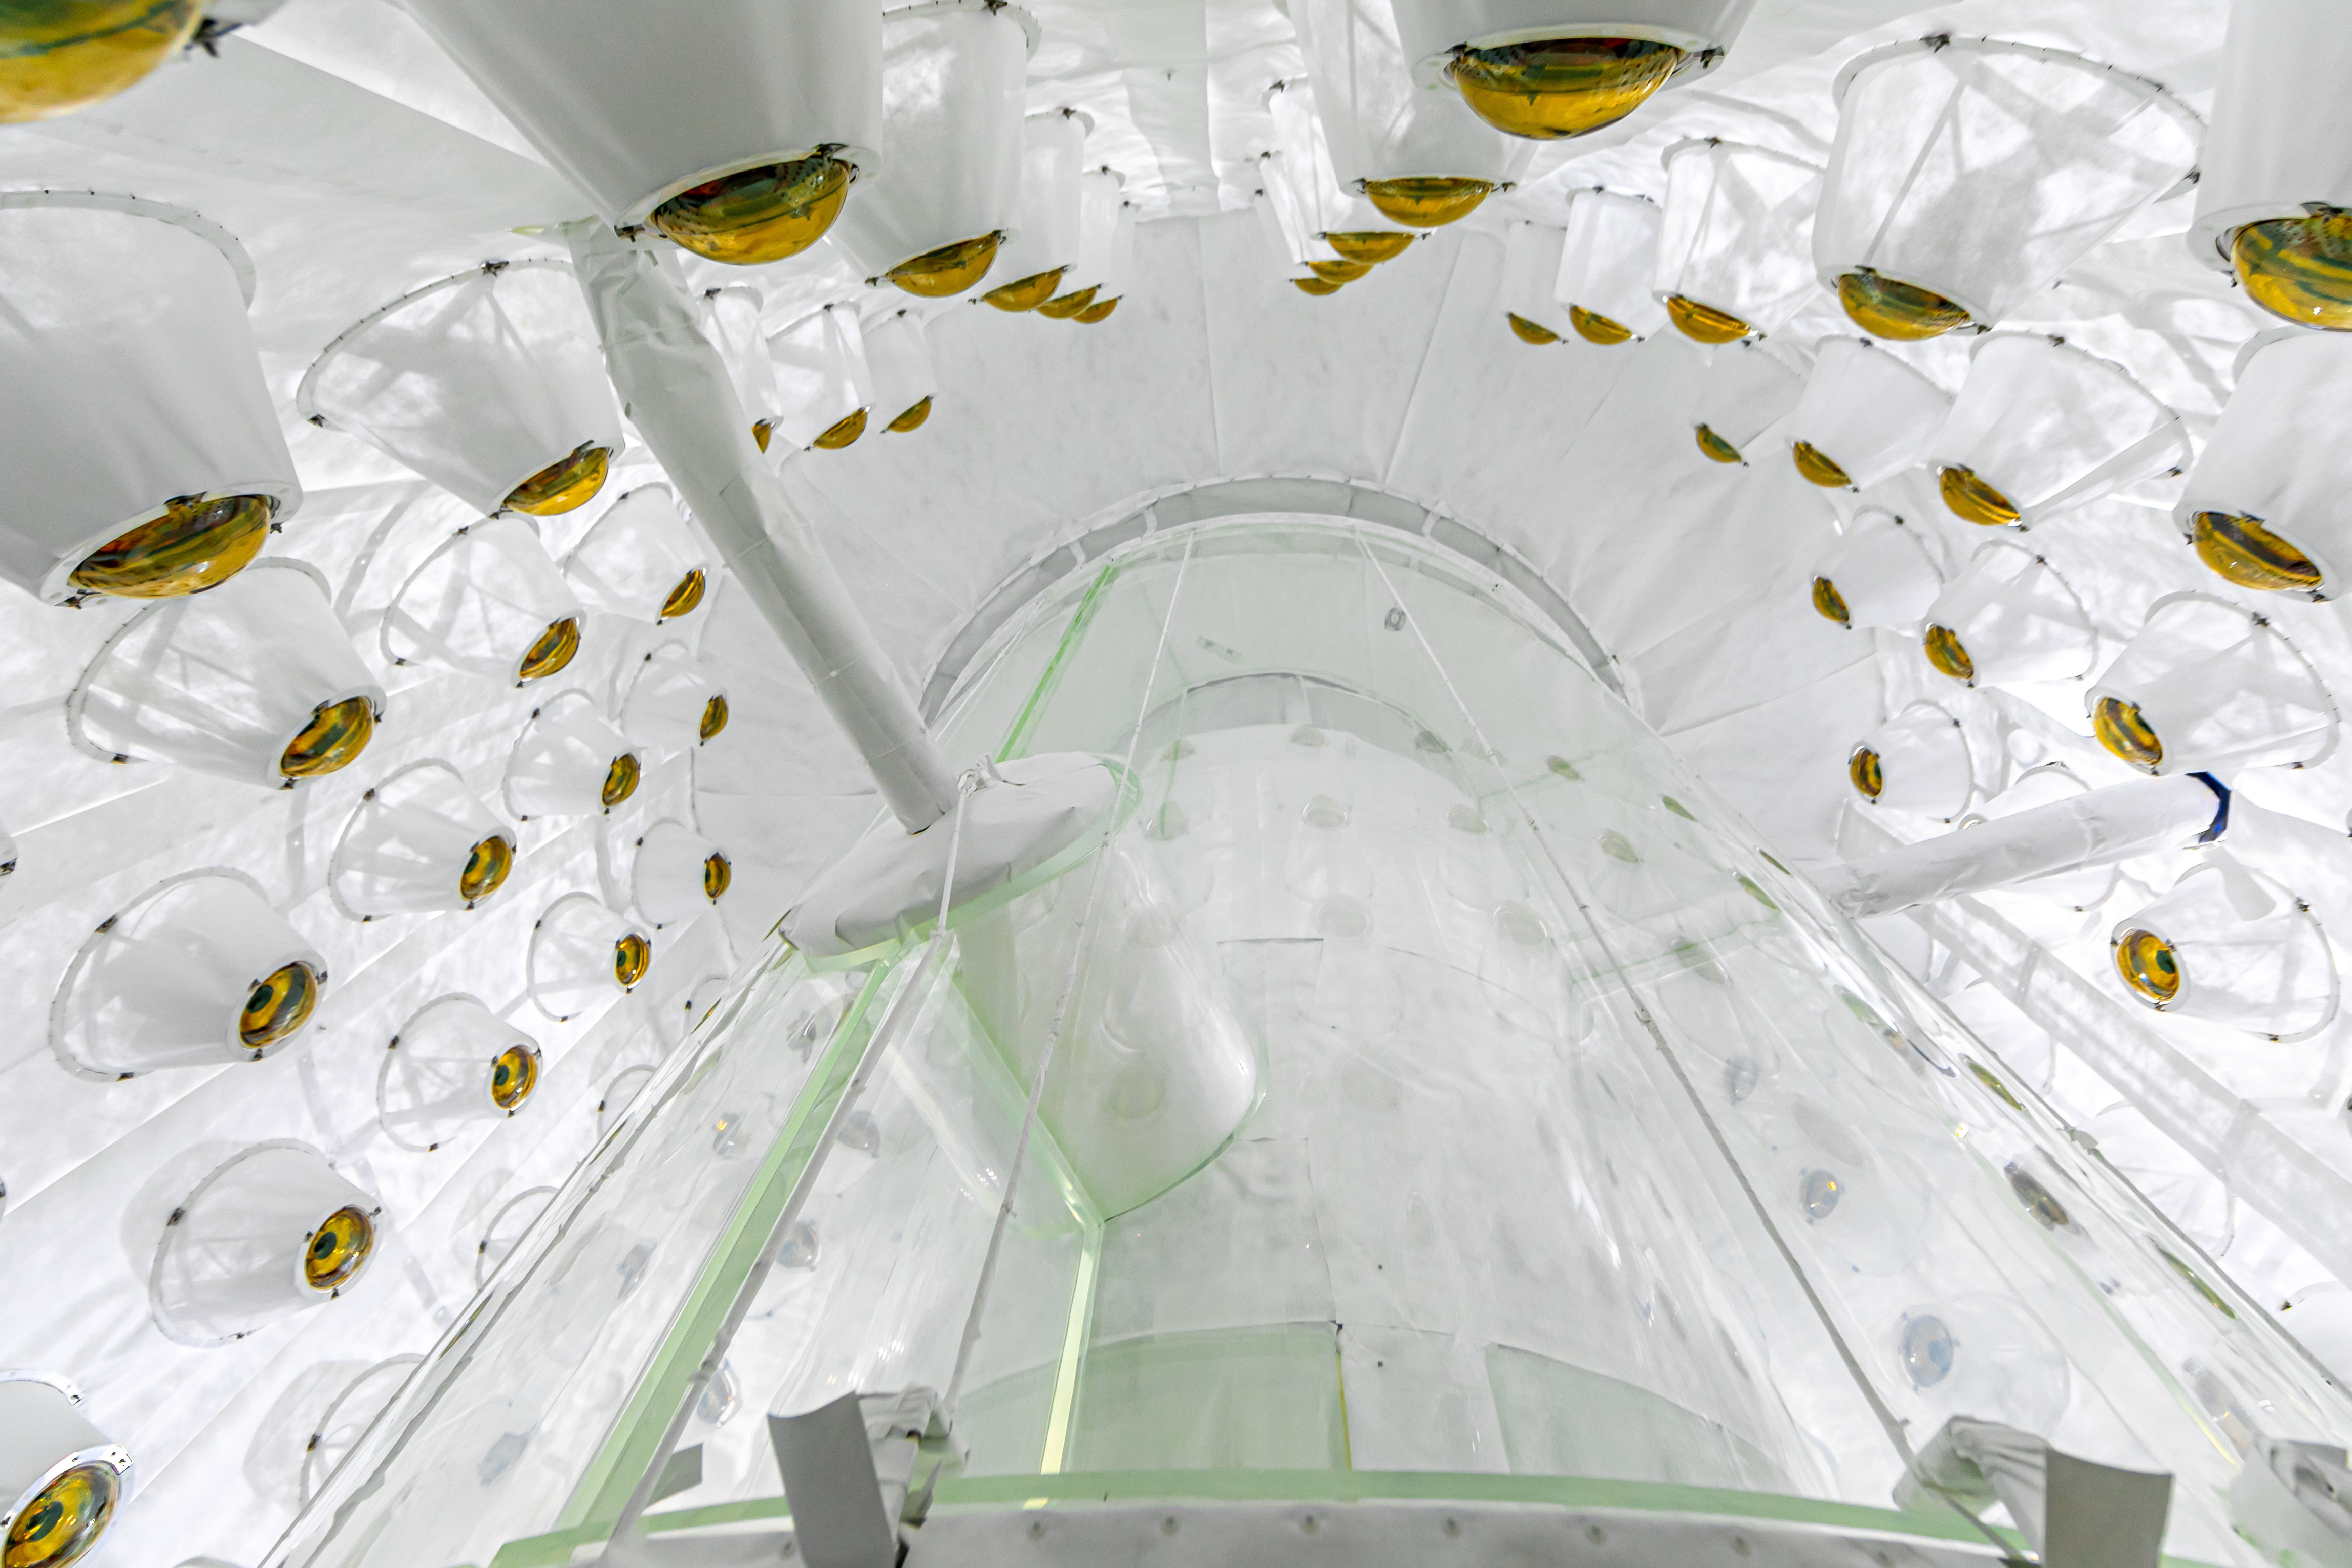
\includegraphics[width=\textwidth]{Figures/Construction/od_complete.jpg}
\centering
\caption{Completed OD installation}
\label{fig:complete_od}
\end{figure}

\par
During the installation described above, the blasting for the Deep Underground Neutrino Experiment (DUNE) began \cite{dune_blasting_ref}.
There was a concern that the pressure change caused by this would damage the tanks.
To stop this, the valves of the tanks were opened whenever there was a planned blast.
This left the inside of each tank open to the cavern-air during this time.

\subsection{Simulation Adaptation}
\par
Many of these design changes, whether it be material or geometrical will have some affect on the performance on the OD.
Most of the changes discussed above have been implemented in the simulation.
A slice through the geometry is shown in Figure \ref{fig:Geometry_Differences} where the differences are highlighted.

\begin{figure}[!htbp]
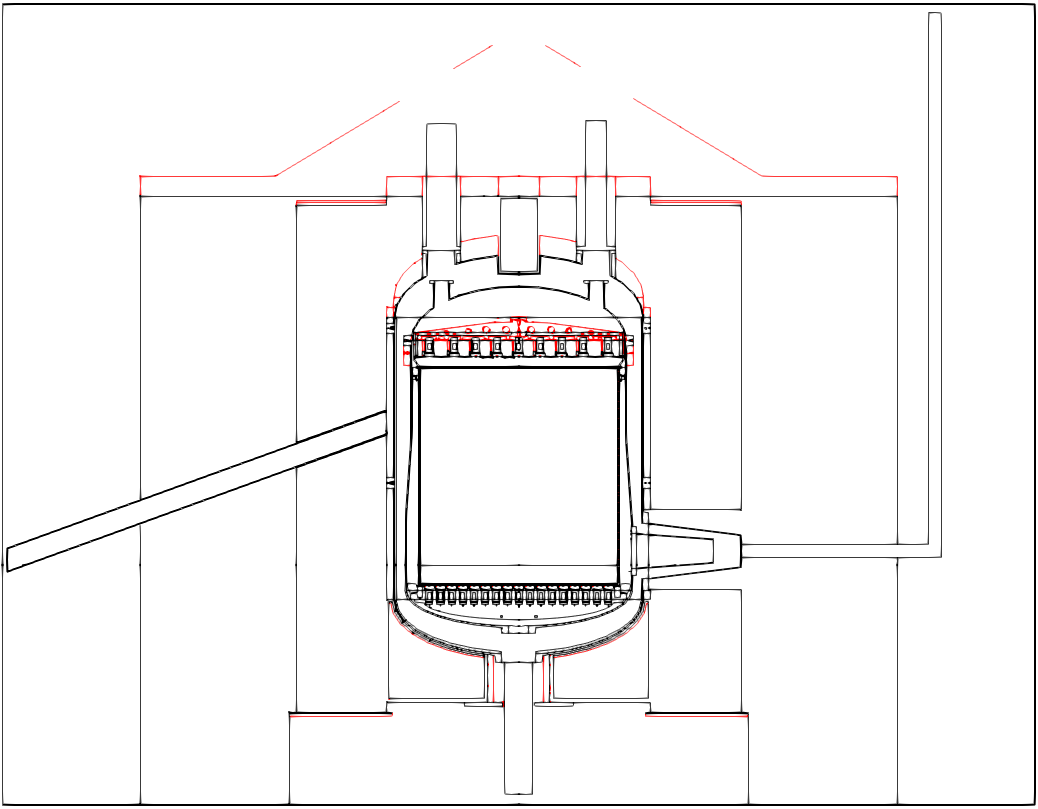
\includegraphics[width=\textwidth]{Figures/Geometry/geometry_differences_black_and_white.png}
\centering
\caption{LZ geometry slice as implemented in Geant4 from the water tank in. In black: the designed geometry as in Figure \ref{fig:LZ_Cut_CAD}. In Red: changes to the design including raised Top OD tanks and additional foam. OD PMTs are not shown here due to none lying on this plane.}
\label{fig:Geometry_Differences}
\end{figure}


%\begin{table}[!htbp]
%    \centering
%    \begin{tabular}{ c | c | c } 
%    \hline
%    \multirow{2}{*}{Volume} & \multicolumn{2}{l}{Percentage captured in volume (\%)} \\ 
%                            & All Neutrons  & SS and FID  \\ \hline
%    volA    & 0.0   & 1232\\
%    volB    & 0.0   &
%    \end{tabular}
%    \caption{Fraction of background neutrons captured in various detector volumes}
%    \label{tab:fraction_of_neutrons_captured_in_volumes}
%\end{table} 